\setcounter{section}{0}
\section{Introduction}

\subsection{Objectives}

\begin{itemize}
\item Learn the difference between compiled and interpreted programming languages.
\item Learn basic facts about Python and its powerful accompanying libraries.
\item Understand how Python programming works in the cloud setting.
\item Write and run your first Python program.
\end{itemize}

\subsection{Compiled and interpreted programming languages}

{\em Compilation} is a process where human-readable {\em source code (text)} is translated by
means of a {\em compiler} and a {\em linker}
into a {\em binary (executable) file} which then can be run on the concrete computer. The same 
source code, compiled on different hardware architectures, yields different binaries. 

{\em Interpreted (scripting)} programming languages are more recent than the compiled ones. 
A program that is written using an interpreted language is "read" (parsed) at runtime -- it is 
not compiled and there are no binaries. Programs 
written using compiled languages are usually more efficient than programs written using the interpreted 
ones because the former take better advantage of the underlying hardware. On the other hand,
interpreted languages are usually more universal and easier to use. Compiled 
programming languages include Pascal, C, C++, Fortran, and many others. Few examples of interpreted 
languages are Python, Lua, Perl and Ruby. 

\subsection{Basic facts about Python}

Python is a powerful modern programming language that is used in many areas of business, 
engineering, and science. Its interpreted character along with a very intuitive syntax make Python an 
ideal language for beginners. 

Python was conceived in the late 1980s and its implementation was started in December 1989
by Guido van Rossum at CWI in the Netherlands. Rossum also gave it a name originated
in his favorite television series {\em Monty Python's Flying Circus}.
Python 2.0 was released in October 2000 and Python 3.0 in December 2008. Python was
awarded the TIOBE {\em Programming Language of the Year} award twice (2007, 2010), which is 
given to the language with the greatest growth in popularity over the course of a year.

Python is a multi-paradigm programming language. Rather than forcing programmers to 
adopt a particular style of programming, it permits several styles: {\em structured (procedural) 
programming} and {\em object-oriented programming} are fully supported, and there are a number 
of language features which support {\em functional programming}. 

In this course you will 
learn the most important aspects of the language and you will be able to 
use the programming language to solve a large variety of problems. 
Depending on your objectives, this course may be all you will ever need. 
We hope that you will like Python and want to learn more -- and there is much 
more to learn out there. References to materials covering more advanced topics 
and object-oriented programming are given in Section \ref{sec:adv}.

\subsection{Libraries - Python programmer's strong companion}

Python comes with a powerful {\em standard library} that contains plentiful functionality
to ease work with constants, types, functions, exceptions, strings, data, 
mathematics, cryptography, parallel processing and other things. 
Python also has a number of scientific libraries. Most important of them are Scipy, 
Numpy, Pylab, Matplotlib, and Sympy.

\subsection{How does Python programming work in the cloud environment?}

In the browser, Python code is typed into one or more input cells in the {\em Python worksheet}. 
The code is sent (as a text string) to a remote server where it is interpreted, and the 
results are sent back to your computer / laptop / tablet, and displayed in your web 
browser.  Let's try this!

\subsection{Launching a Python project}

There are multiple ways to launch a Python project. First, it is 
possible to clone and experiment with many existing displayed Python 
projects via File Manager $\rightarrow$ 
Project $\rightarrow$ Clone. New (empty) Python project can be launched via 
the {\em Programming} menu or via File Manager $\rightarrow$ 
Project $\rightarrow$ New $\rightarrow$ Python. An empty Python worksheet
is shown in Fig. \ref{fig:python}.

\newpage
\begin{figure}[!ht]
\begin{center}
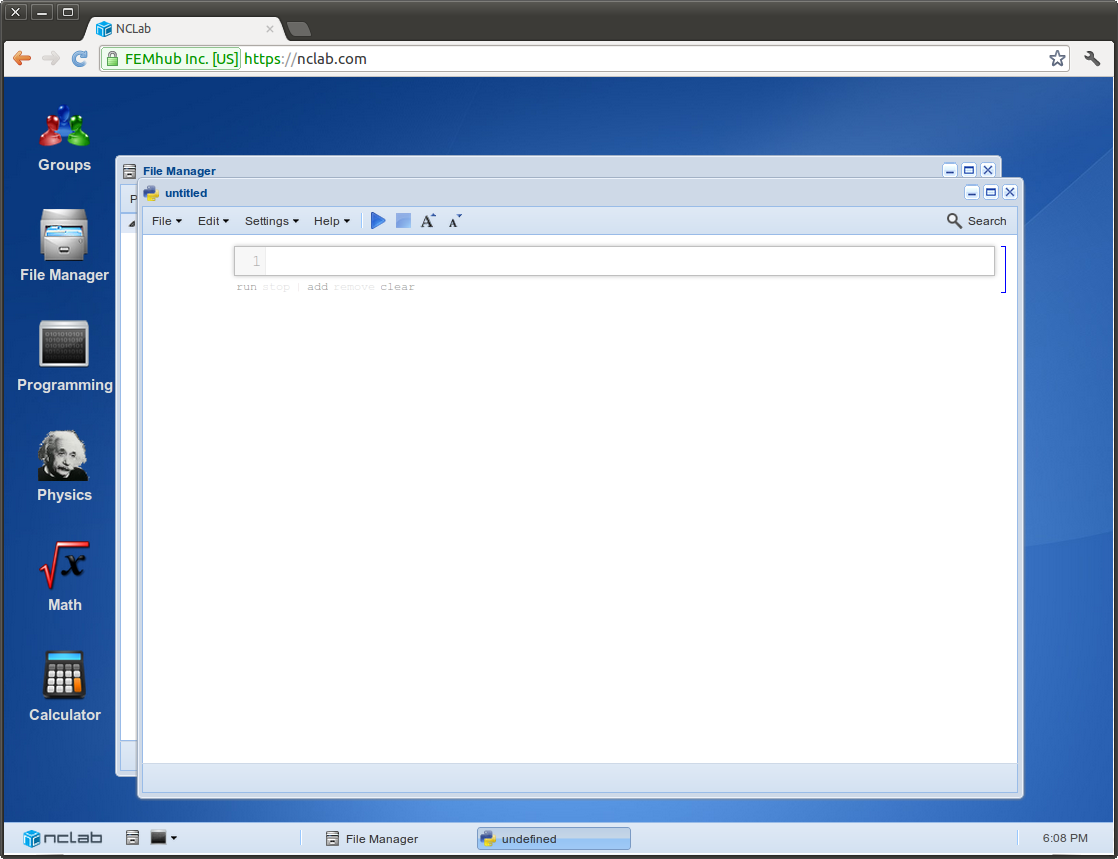
\includegraphics[width=0.9\textwidth]{imgp/python.png}
\end{center}
\vspace{-2mm}
\caption{Launching a new Python project.}
\label{fig:python}
\end{figure}


\subsection{Hello, World!}

Click into the input cell and type {\tt print "Hello, World!"}.
Then click on {\tt run} link under the input cell, and the text 
"Hello, World!" will be displayed 
in a new yellow {\em output cell} as shown in Fig. \ref{fig:python-2}.

\newpage

\begin{figure}[!ht]
\begin{center}
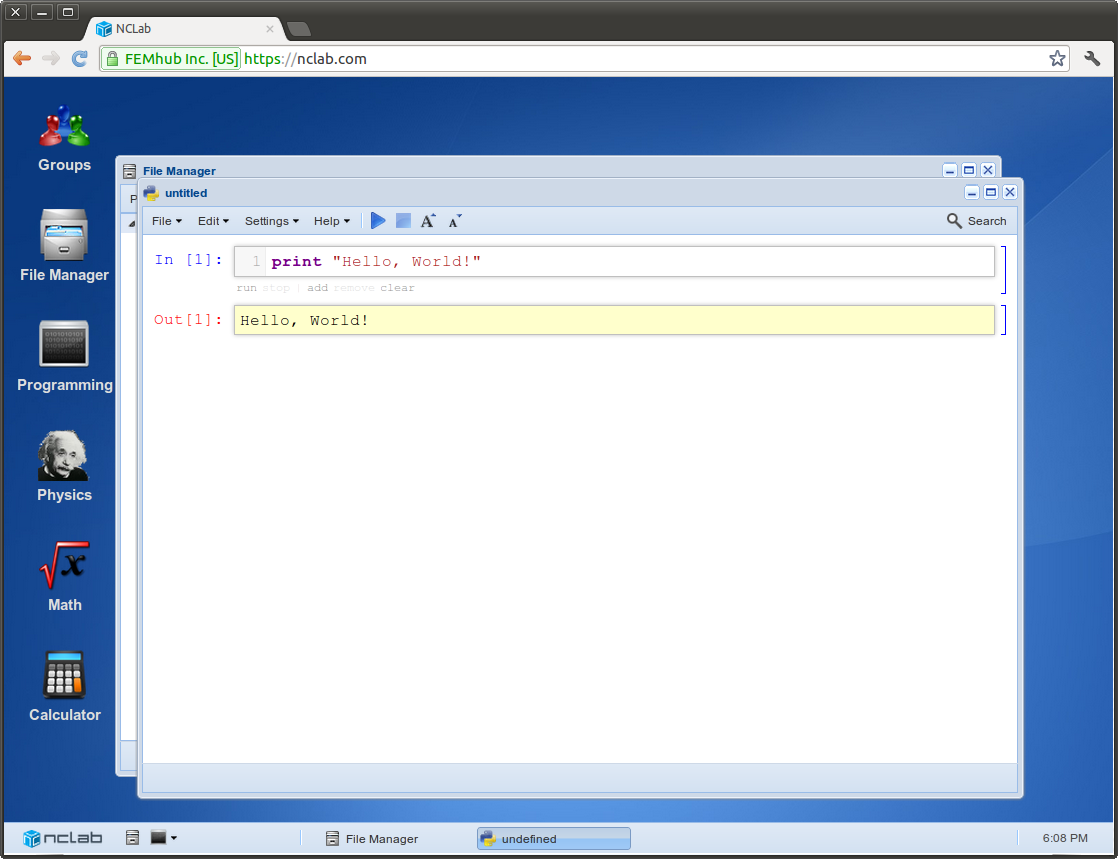
\includegraphics[width=0.9\textwidth]{imgp/python-2.png}
\end{center}
\vspace{-2mm}
\caption{Response received from the cloud is shown in a yellow output cell.}
\label{fig:python-2}
\end{figure}

\subsection{Input, output and text cells}

As in Karel, there are three types of cells in the Python worksheet - input cells, output cells, 
and descriptive text cells. Input cells as well as text cells can be added via 
the {\em Edit} menu. New input cells can be also added easily by clicking on {\tt add} under
an existing input cell. Input cells and text cells can be removed by clicking on 
{\tt remove} under them. The easiest way to remove a selected output cell is to 
click on it with the mouse and press DELETE on the keyboard. 
All output cells can be removed at once via {\em Remove all output} in the {\em Edit} menu. 

\subsection{Various ways to run programs}

Pressing the blue arrow button will run all input cells in the project. Clicking 
on {\tt run} under an input cell will run only the contents of that input cell. 
Same effect can be achieved by holding CTRL and pressing ENTER. Holding SHIFT
and pressing ENTER will evaluate the current input cell and create an additional one
under it.

\subsection{\ \ Review questions}

As in the first part of the textbook, one or more answers can be correct. 
\begin{enumerate}
\item What is the difference between a compiled and a scripting programming language?
\begin{enumerate}
\item[A1] Programs written in compiled languages are binary files. 
\item[A2] Compiled languages are easier to use than the scripting ones.
\item[A3] Programs written in scripting languages are usually more efficient than programs 
          written in the compiled ones.
\item[A4] Scripting languages do not require a compiler.
\end{enumerate}
\item What languages take better advantage of the underlying hardware architecture
      and why?
\begin{enumerate}
\item[A1] Scripting languages because they are less hardware-dependent.
\item[A2] Compiled languages because the executable files are tailored 
          to the concrete hardware.
\item[A3] Compiled languages because  they do not require a linker.
\item[A4] Scripting languages because they do not require a compiler.
\end{enumerate}
\item Give three examples of compiled programming languages.
\begin{enumerate}
\item[A1] Fortran, C++ and Lua.
\item[A2] Python, Ruby and C.
\item[A3] C, C++ and Fortran.
\item[A4] Python, Lua and Perl.
\end{enumerate}
\item Give three examples of interpreted programming languages.
\begin{enumerate}
\item[A1] Pascal, Perl and Python.
\item[A2] Lua, C and C++.
\item[A3] Perl, Python and Ruby. 
\item[A4] C, C++ and Fortran.
\end{enumerate}
\item Where does the name "Python" of the programming language come from?
\begin{enumerate}
\item[A1] The snake, {\em Python regius}.
\item[A2] TV show in Great Britain.
\item[A3] Recognized brand name of remote start systems.
\item[A4] Recognized brand name of aquarium products.
\end{enumerate}
\item When was the implementation of Python started?
\begin{enumerate}
\item[A1] 1989
\item[A2] 1995
\item[A3] 2000
\item[A4] 2005
\end{enumerate}
\item Name three programming styles that Python permits.
\begin{enumerate}
\item[A1] Compiled, interpreted, scripting.
\item[A2] Structured, object-oriented, functional.
\item[A3] Procedural, object-oriented, binary.
\item[A4] Good, bad, ugly.
\end{enumerate}
\item How can displayed Python projects be cloned?
\begin{enumerate}
\item[A1] In Python worksheet through the {\em File} menu.
\item[A2] Through File Manager's {\em Project} menu.
\item[A3] Using the icon {\em Displayed projects} on Desktop.
\item[A4] Python projects cannot be cloned.
\end{enumerate}
\item How can new Python project be launched?
\begin{enumerate}
\item[A1] Through the {\em Programming} menu.
\item[A2] Through File Manager's {\em Settings} menu.
\item[A3] Through File Manager's {\em Project} menu.
\item[A4] Through the Math module.
\end{enumerate}
\item How are Python programs processed?
\begin{enumerate}
\item[A1] They are translated into Javascript and run as a standard web browser application.
\item[A2] They are interpreted on a remote server.
\item[A3] They are interpreted on your PC computer / laptop / tablet.
\item[A4] They are translated into Flash.
\end{enumerate}
\item What are the types of cells that a Python worksheet can contain?
\begin{enumerate}
\item[A1] Error message cells.
\item[A2] Output cells.
\item[A3] Input cells.
\item[A4] Descriptive text cells.
\end{enumerate}
\item How can all input cells in a Python worksheet be evaluated at once?
\begin{enumerate}
\item[A1] By typing Evaluate in the last input cell and hitting ENTER.
\item[A2] By clicking on {\tt run} under the last input cell.
\item[A3] By clicking on {\em Evaluate all} in the {\em File} menu. 
\item[A4] By clicking on the blue arrow button in the menu.
\end{enumerate}
\item How can a single input cell be evaluated?
\begin{enumerate}
\item[A1] By clicking on {\tt save} under the input cell.
\item[A2] By clicking on the blue arrow button in the menu.
\item[A3] By clicking on {\tt run} under the input cell.
\item[A4] By clicking on the blue square button in the menu.
\end{enumerate}
\item What is the way to add a new input cell?
\begin{enumerate}
\item[A1] Click on {\tt add} under an input cell. 
\item[A2] Click on {\em New} in the {\em File} menu.
\item[A3] Click on the larger "A" icon in the menu.
\item[A4] Click on {\em New input cell} in {\em Edit} menu.
\end{enumerate}
\item How can a new text cell be added?
\begin{enumerate}
\item[A1] Click on {\tt add} under an input cell. 
\item[A2] Click on {\em New text cell} in the {\em Edit} menu.
\item[A3] Click on {\em New} in the {\em File} menu.
\item[A4] Click on the smaller "A" icon in the menu.
\end{enumerate}
\item What is the way to remove an input cell or a text cell?
\begin{enumerate}
\item[A1] Click on {\tt remove} under the cell. 
\item[A2] Click on {\tt clear} under the cell. 
\item[A3] Click on {\em Clear active cell} in the {\em Edit} menu.
\item[A4] Click on {\em Close} in the {\em File} menu.
\end{enumerate}
\item How can an input cell be evaluated without using the mouse?
\begin{enumerate}
\item[A1] Hold CTRL and press ENTER.
\item[A2] Hold SHIFT and press ENTER.
\item[A3] Press ENTER twice.
\item[A4] Press CTRL + ALT + SHIFT.
\end{enumerate}
\item Which of the following are scientific libraries for Python?
\begin{enumerate}
\item[A1] GNU Scientific Library.
\item[A2] Numpy.
\item[A3] Scipy.
\item[A4] Sympy.
\end{enumerate}
\end{enumerate}

\subsection{\ \ Programming exercises}

\begin{enumerate}
\item Write a Python program that prints your name. Run it by clicking on the blue arrow button.
\item Write a Python program that prints the name of your favorite animal. 
      Run it by clicking on {\tt run} under the input cell.
\item Write a Python program that prints the name of your favorite singer 
      or music band. Run it without using the mouse.
\end{enumerate}

\section{Using Python as a graphing calculator} \label{sec:calc}

\subsection{Objectives}

\begin{itemize}
\item Learn how to use Python for advanced math operations.
\item Plotting graphs of functions of one and two variables, as well as parametric 2D and 3D curves.
\end{itemize}
The Python worksheet can be used as a powerful calculator and graphing utility. 
Let us begin with the simplest math operations.

\subsection{Addition, subtraction}

Launch a new Python project and in the input cell type:

\begin{verbatim}
3 + 6
\end{verbatim}
Then click on the {\tt run} link under the input cell. The output should be displayed quickly:

\begin{verbatim}
9
\end{verbatim}
You can add real numbers too,
\begin{verbatim}
3.2 + 6.31
\end{verbatim}
Output:

\begin{verbatim}
9.51
\end{verbatim}
Two numbers can be subtracted as follows,

\begin{verbatim}
7.5 - 2.1
\end{verbatim}
Output:

\begin{verbatim}
5.4
\end{verbatim}

\subsection{Multiplication}
Multiplication is done using the '{\tt *}' symbol as in

\begin{verbatim}
3 * 12
\end{verbatim}
Output:

\begin{verbatim}
36
\end{verbatim}
Of course, real numbers can be multiplied as well:

\begin{verbatim}
3.7 * 12.17
\end{verbatim}
Output:

\begin{verbatim}
45.029
\end{verbatim}
\subsection{Division}
With division, we need to be a bit careful. Look at this:

\begin{verbatim}
30 / 5
\end{verbatim}
Output:

\begin{verbatim}
6
\end{verbatim}
And then look at this:

\begin{verbatim}
33 / 5
\end{verbatim}
Output:

\begin{verbatim}
6
\end{verbatim}
In all major computer languages including C, C++, Fortran, Python and 
others:\\

\begin{center}
\framebox{\color{red}\bf The result of division of two integers is an integer!}
\end{center}

\vspace{4mm}
\noindent
So, when dividing two integers, everything behind the decimal point is lost.
In order to stay on the safe side, 
before you perform division of two numbers, always convert at least one of them
to a real number. This is simple: While {\tt 5} is an integer, {\tt 5.}
and {\tt 5.0} are reals. It is also possible to 
say {\tt float(5)}. In fact this is the best way since it also works for 
variables. Such as, when we are dividing {\tt a / b}, to make sure that 
the result will be correct also for integers, we type {\tt float(a) / b}. 
When at least one number is a real, then the result of the division is a real.   
Variables will be discussed shortly.

\subsection{Powers}
Sometimes we need to use exponents, such as in $2^4$. Python has a double-star
symbol {\tt **} for this:

\begin{verbatim}
2**4
\end{verbatim}
Output:

\begin{verbatim}
16
\end{verbatim}
\subsection{Modulo}
The last of the common arithmetic operations is {\em modulo}. Recall that this is the remainder 
after integer division. In Python modulo is done using the per cent symbol:

\begin{verbatim}
6 % 4
\end{verbatim}
Output:

\begin{verbatim}
2
\end{verbatim}
Of course, one can use brackets:

\begin{verbatim}
5 * (7 - 3)
\end{verbatim}
Output:

\begin{verbatim}
20
\end{verbatim}
\subsection{Order of operations}
Python respects the standard order of operations:

\begin{itemize} 
\item Round brackets have the highest priority,
\item then exponentiation, 
\item then multiplication and division (same priority),
\item the lowest priority have addition and subtraction.
\end{itemize}
Note that no other brackets such as {\tt \{ \}} and {\tt [ ]} are 
admissible in mathematical expressions since they have a different 
function in the programming language.

To illustrate the priority of operations, we can try the following:

\begin{verbatim}
3**4 / 27 * 5 + 3 * 5
\end{verbatim}
Output:

\begin{verbatim}
30
\end{verbatim}
\subsection{Using empty characters makes you code better readable}
Your code will be much better readable if you use empty
characters on either side of arithmetic symbols, as well as 
after commas. Hence, you should never write things like {\tt 3**4/27*5+3*5}.

\subsection{Using mathematical functions}

In order to calculate square roots, exponentials, sines, cosines, tangents, and many other 
math functions, the best way is to import Numpy. Numpy is a powerful Python library 
for numerical computations. To import it, just include the following 
line in your code:

\begin{verbatim}
from numpy import *
\end{verbatim}
Here the symbol '{\tt *}' stands for "everything". If you wanted to import just one or two 
functions, you could do that as well by just giving their names, separated by commas. 

After Numpy is imported, we can calculate, for example, $e^2$:

\begin{verbatim}
exp(2)
\end{verbatim}
Output:
\begin{verbatim}
7.3890560989306504
\end{verbatim}
Elementary functions (and constants) that one can import from Numpy are listed
below. We also show their arguments for clarity, but the functions are imported without 
them. For example, the absolute value function is imported via {\tt from numpy import abs}.\\

%{\small
\begin{center}
\begin{tabular}{|l|l|}
\hline
pi &  $\pi$\\
abs($x$) &  absolute value of $x$\\
arccos($x$) &  inverse cosine of $x$ \\
arccosh($x$) &  inverse hyperbolic cosine of $x$ \\
arcsin($x$) & inverse sine of $x$ \\
arcsinh($x$) & inverse hyperbolic sine of $x$ \\
arctan($x$) & inverse tangent of $x$ \\
arctanh($x$) & inverse hyperbolic tangent of $x$ \\
arctan2($x_1$, $x_2$) & arc tangent of $x_1/x_2$ choosing the quadrant correctly \\
cos($x$) & cosine of $x$ \\
cosh($x$) & hyperbolic tangent of $x$ \\
exp($x$) & $e^x$ \\
log($x$) & natural logarithm of $x$ \\
pow($a$, $b$) & $a^b$ (same as "a**b")\\
sin($x$) & sine of $x$ \\
sinh($x$) & hyperbolic sine of $x$ \\
sqrt($x$) & square root of $x$ \\
tan($x$) & tangent of $x$\\
tanh($x$) & hyperbolic tangent of $x$ \\
\hline
\end{tabular}
\end{center}
%}
\vspace{4mm}
\noindent

\subsection{\ \ Complex numbers}
Complex numbers are always represented as two floating point numbers, the 
real and imaginary part. Appending '{\tt j}' or  '{\tt J}' to a real number
makes it imaginary:

\begin{verbatim}
1j * 1J
\end{verbatim}
Output:

\begin{verbatim}
(-1+0j)
\end{verbatim}
This is one way to define complex numbers:
\begin{verbatim}
1 + 3j
\end{verbatim}
Output:

\begin{verbatim}
(1+3j)
\end{verbatim}
Another way is to use the command {\tt complex}:

\begin{verbatim}
complex(1, 3)
\end{verbatim}
Output:

\begin{verbatim}
(1+3j)
\end{verbatim}
All arithmetic operations that are used for real numbers can be 
used for complex numbers as well, for example:

\begin{verbatim}
(1 + 2j) / (1 + 1j)
\end{verbatim}
Output:

\begin{verbatim}
(1.5+0.5j)
\end{verbatim}
To extract the real and imaginary parts of a complex number {\tt z}, use {\tt z.real}
and {\tt z.imag}. Use {\tt abs()} to get the absolute value:

\begin{verbatim}
a = 3 + 4j
a.real
a.imag
abs(a)
\end{verbatim}
Output:

\begin{verbatim}
3
4
5
\end{verbatim}


\subsection{\ \ Plotting functions of one variable}\label{plotting}

Plotting can be done via the Pylab library. The Pylab {\tt plot} command takes two
arrays: $x$-coordinates and $y$-coordinates of points on a curve. Between the 
points, the curve is interpolated linearly. Let us illustrate this on a simple 
example with just five points [0, 0], [1, 2], [2, 0.5], [3, 2.5] and [4, 0]:

\begin{verbatim}
from pylab import *
x = [0,0, 1.0, 2.0, 3.0, 4.0]
y = [0.0, 2.0, 0.5, 2.5, 0]
clf()
plot(x, y)
lab.show()
\end{verbatim}
The commands {\tt clf()}, {\tt plot()} and {\tt lab.show()} do clear the canvas, 
plot the graph, and show the graph, respectively.
The output is shown in Fig. \ref{fig:plot}.


\begin{figure}[!ht]
\begin{center}
\hbox{}
\hspace{-6mm}
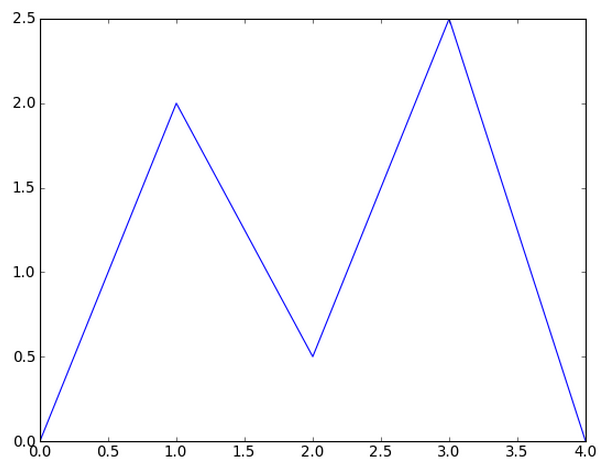
\includegraphics[width=0.56\textwidth]{imgp/plot.png}
\end{center}
\vspace{-2mm}
\caption{Piecewise-linear curve with five points.}
\label{fig:plot}
%\vspace{-1cm}
\end{figure}
\noindent
In the following we will discuss more options and show some useful techniques.
Let's say, for example, that we want to plot the function $f(x) = \sin(x)$
in the interval $(0, 2\pi)$. The array of $x$-coordinates of equidistant points 
between 0 and $\pi$ with step 0.05 can be created easily using the command {\tt arange}:

\begin{verbatim}
from numpy import *
x = arange(0, 2*pi, 0.05)
\end{verbatim}
Changing the step size will change the resolution - with a smaller step the resolution will 
be finer and vice-versa. Next, the array of $y$-coordinates of the points is obtained via

\begin{verbatim}
y = sin(x)
\end{verbatim}
The last part we already know:

\begin{verbatim}
clf()
plot(x, y)
lab.show()
\end{verbatim}
\noindent
The output is shown in Fig. \ref{fig:plot1}.\\[-7mm]

\begin{figure}[!ht]
\begin{center}
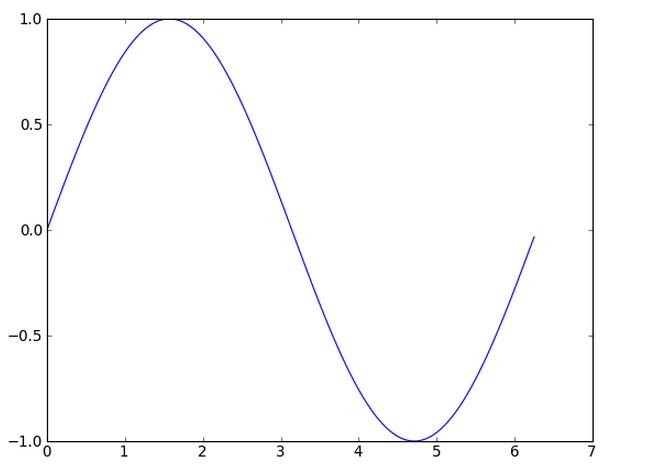
\includegraphics[width=0.6\textwidth]{imgp/plot1.png}
\end{center}
\vspace{-6mm}
\caption{Plotting $\sin(x)$ in interval $(0, 2\pi)$ with subdivision step 0.05.}
\label{fig:plot1}
\vspace{-2mm}
\end{figure}
\noindent

\subsection{\ \ Labels, colors, and styles}

The plot can be made nicer by adding a label, and also the color 
and the line style can be changed. Let us start with adding a label:

\begin{verbatim}
plot(x, y, 'b-', label = "Solid blue line")
legend()
lab.show()
\end{verbatim}
The output is shown in Fig. \ref{fig:plot2}.\\[-7mm]

\begin{figure}[!ht]
\begin{center}
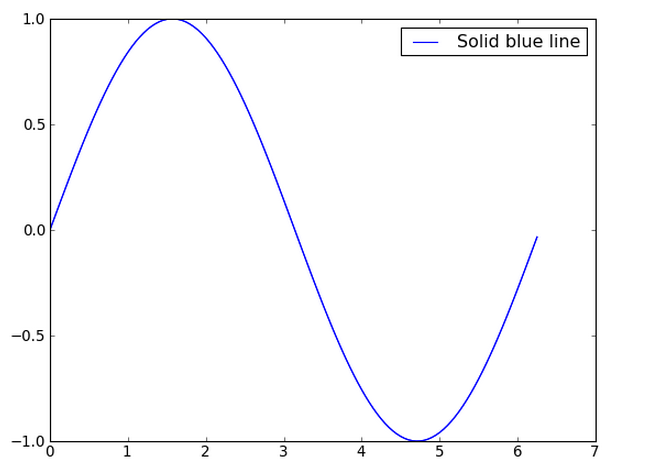
\includegraphics[width=0.6\textwidth]{imgp/plot2.png}
\end{center}
\vspace{-6mm}
\caption{Adding a label.}
\label{fig:plot2}
%\vspace{-1cm}
\end{figure}
\newpage
\noindent
Next let us change the color to red and line style to dashed: 

\begin{verbatim}
clf()
plot(x, y, 'r--', label = "Dashed red line")
legend()
lab.show()
\end{verbatim}
The output is shown in Fig. \ref{fig:plot3}.\\[-7mm]


\begin{figure}[!ht]
\begin{center}
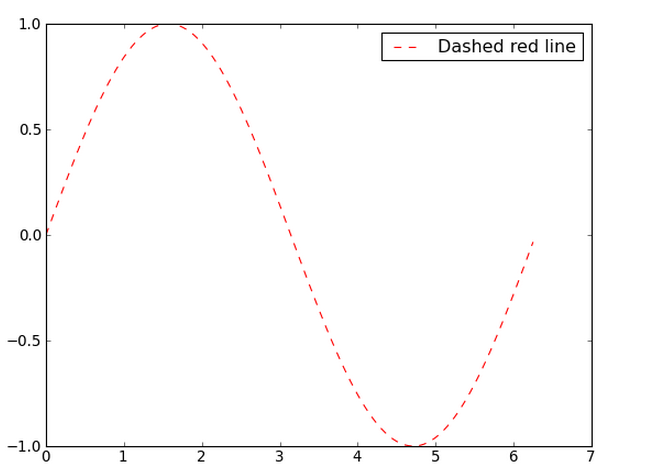
\includegraphics[width=0.6\textwidth]{imgp/plot3.png}
\end{center}
\vspace{-6mm}
\caption{Same graph using dashed red line.}
\vspace{-1cm}
\label{fig:plot3}
\end{figure}
\newpage
\noindent
The graph can be plotted using green color and small dots rather than 
a solid or dashed line:

\begin{verbatim}
clf()
plot(x, y, 'g.', label = "Dotted green line")
legend()
lab.show()
\end{verbatim}
The output is shown in Fig. \ref{fig:plot4}.

\begin{figure}[!ht]
\begin{center}
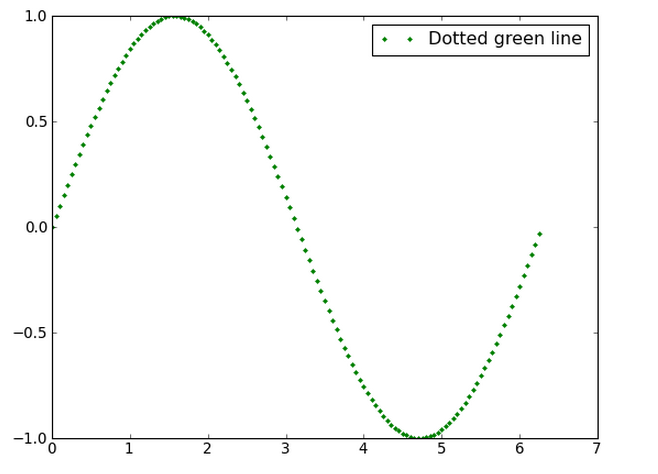
\includegraphics[width=0.6\textwidth]{imgp/plot4.png}
\end{center}
\vspace{-6mm}
\caption{Same graph using dotted green line.}
\label{fig:plot4}
%\vspace{-5mm}
\end{figure}
\noindent
\noindent
Last let us stay with green color but make the dots larger:

\begin{verbatim}
clf()
plot(x, y, 'go', label = "Bigger green dots")
legend()
lab.show()
\end{verbatim}
\noindent
The output is shown in Fig. \ref{fig:plot5}.
\newpage

\begin{figure}[!ht]
\begin{center}
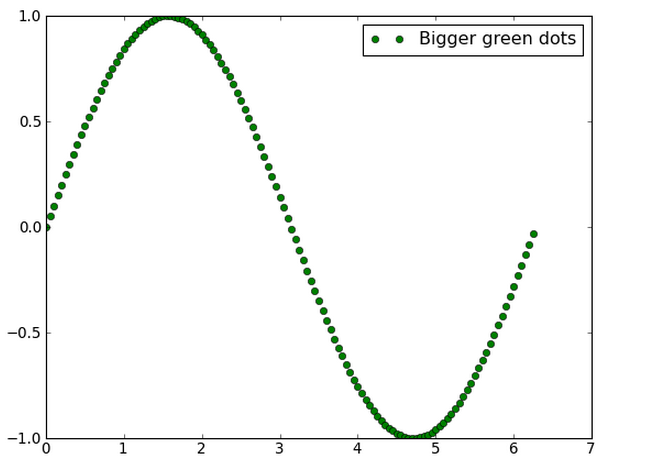
\includegraphics[width=0.6\textwidth]{imgp/plot5.png}
\end{center}
\vspace{-6mm}
\caption{Same graph using large green dots.}
\label{fig:plot5}
%\vspace{-4mm}
\end{figure}
\noindent

\subsection{\ \ Scaling axes and showing grid}

In the previous plots, function graphs were fitted into the 
display window, which means that the horizontal and vertical 
axes were scaled differently. This can be changed by including the 
{\tt axis('equal')} command after calling {\tt plot()}. Also, 
grid can be displayed by using the {\tt grid()} command:

\begin{verbatim}
from numpy import *
from pylab import *
x = arange(0, 2*pi, 0.05)
y = sin(x)
clf()
plot(x, y, label="sin(x)")
axis('equal')
grid()
legend()
lab.show()
\end{verbatim}
\noindent
The output is shown in Fig. \ref{fig:plot8}.
\newpage

\begin{figure}[!ht]
\begin{center}
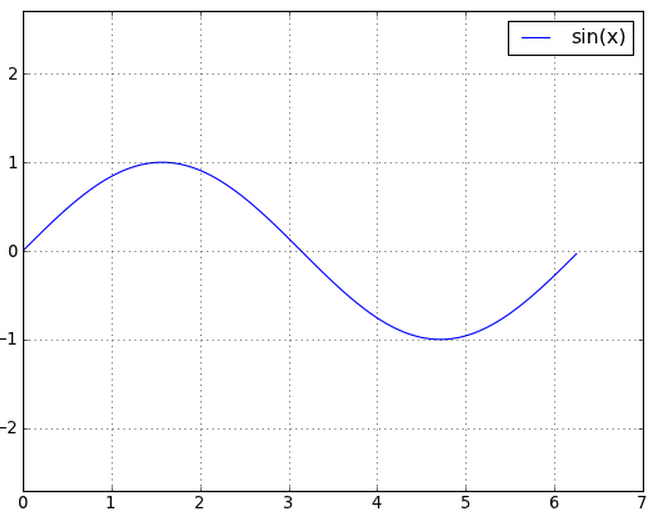
\includegraphics[width=0.53\textwidth]{imgp/plot8.png}
\end{center}
\vspace{-4mm}
\caption{Scaling axes equally and showing grid.}
\label{fig:plot8}
\vspace{-2mm}
\end{figure}
\noindent
The scaling of axes can be returned to the automatic fit option via
{\tt axis('auto')} if needed.

\subsection{\ \ Adjusting plot limits}

Plot limits can be set using the {\tt xlim()} and {\tt ylim()}
functions after {\tt plot()}. For example, we can stretch the sine
function from Fig. \ref{fig:plot8} to span the entire width of the 
canvas as follows:

\begin{verbatim}
from numpy import *
from pylab import *
x = arange(0, 2*pi, 0.05)
y = sin(x)
clf()
plot(x, y, label="sin(x)")
xlim(0, 2*pi)
axis('equal')
grid()
legend()
lab.show()
\end{verbatim}
\noindent
The output is shown in Fig. \ref{fig:plot9}.
\newpage

\begin{figure}[!ht]
\begin{center}
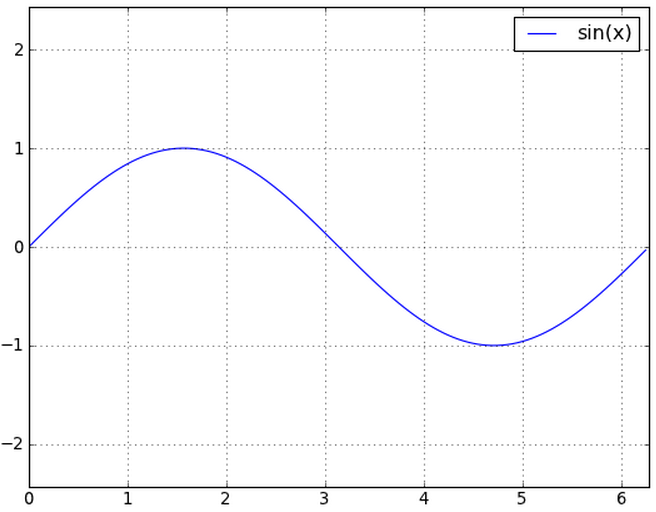
\includegraphics[width=0.53\textwidth]{imgp/plot9.png}
\end{center}
\vspace{-4mm}
\caption{Setting plot linits on the horizontal axis to $0$ and $2\pi$.}
\label{fig:plot9}
\vspace{-2mm}
\end{figure}
\noindent


\subsection{\ \ Plotting multiple functions at once}

This can be done very easily, just do not use the {\tt clf()}
command between the plots and you can have as many graphs 
in one figure as needed. Let us do three:

\begin{verbatim}
from numpy import *
from pylab import *
x = arange(0.5, 5, 0.05)
y1 = 1./x
y2 = 1. / (1 + x**2)
y3 = exp(-x)
axis=("equal")
clf()
plot(x, y1, label="y1")
plot(x, y2, label="y2")
plot(x, y3, label="y3")
legend()
lab.show()
\end{verbatim}
\noindent
The output is shown in Fig. \ref{fig:plot7}.
\newpage

\begin{figure}[!ht]
\begin{center}
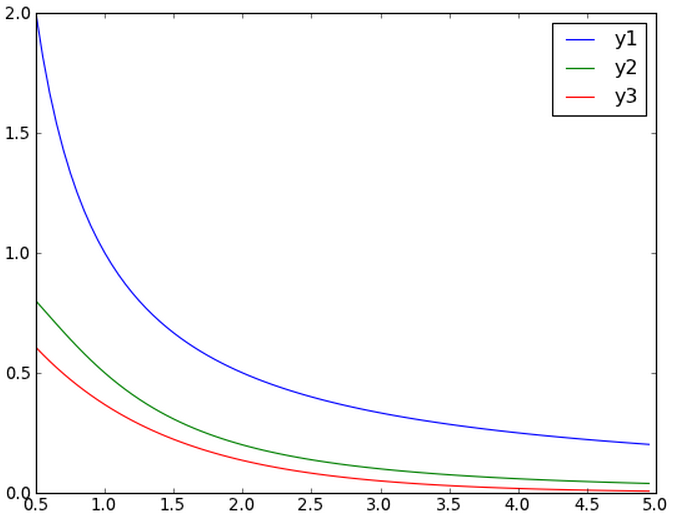
\includegraphics[width=0.54\textwidth]{imgp/plot7.png}
\end{center}
\vspace{-4mm}
\caption{Plotting graphs of functions $1/x$, $1 / (1 + x^2)$ and $e^{-x}$ in interval $(0.5, 5)$.}
\label{fig:plot7}
\vspace{-2mm}
\end{figure}
\noindent
The {\tt plot()} command in Pylab is much more powerful, we just saw a small 
fraction of its functionality. For a complete list of options 
visit the Pylab page {\tt http:// www.scipy.org/PyLab}.

\subsection{\ \ Plotting parametric 2D curves}\label{subsec:planarcurves}

The concept of plotting based on two arrays of $x$ and $y$ coordinates
allows us to do much more than only plot graphs of functions of one variable.
We can easily plot more general curves such as circles, spirals and others.
Let us illustrate this on a spiral that is parameterized 
by 
$$
x(t) = t \cos(t), \ \ \ \ 
y(t) = t \sin(t)
$$ 
in the interval $(0, 10)$ for $t$. The complete code is

\begin{verbatim}
from pylab import *
from numpy import *
t = arange(0, 10, 0.05)
x = t*cos(t)
y = t*sin(t)
clf()
plot(x, y)
lab.show()
\end{verbatim}
The output is shown in Fig. \ref{fig:plot6}.

\begin{figure}[!ht]
\begin{center}
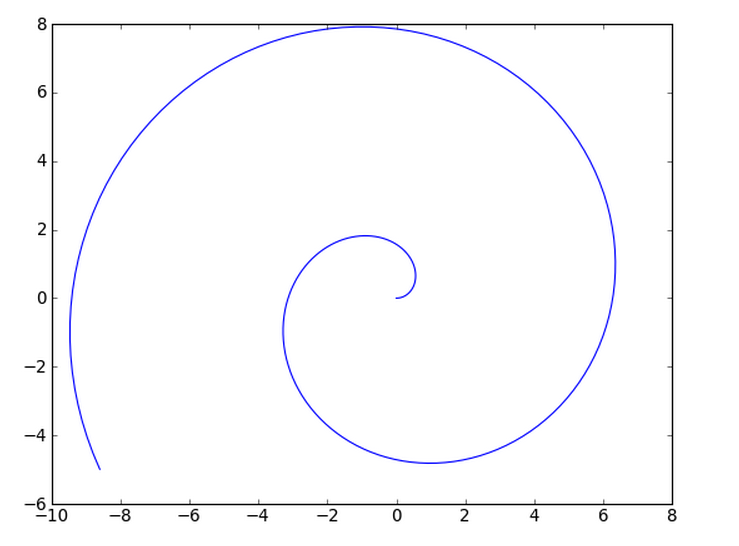
\includegraphics[width=0.6\textwidth]{imgp/plot6.png}
\end{center}
\vspace{-6mm}
\caption{Plotting a spiral.}
\label{fig:plot6}
\vspace{-0mm}
\end{figure}
\noindent

\subsection{\ \ Plotting parametric 3D curves}

For 3D plots it is practical to use the {\tt mplot3d} toolkit of the 
Python library Matplotlib. Let us begin with 
parametric 3D curves since this is analogous to how we handled planar curves in 
the previous paragraph. 3D curves are sequences of linearly interpolated 3D points
represented via three arrays of $x$, $y$ and $z$ coordinates. As an 
example we will plot the curve $x(t), y(t), z(t)$ where

$$
x(t) = (1 + t^2) \sin(2 \pi t), \ \ \ y(t) = (1 + t^2) \cos(2 \pi t), \ \ \ z(t) = t,
$$
and where the parameter $t$ lies in the interval $(-2, 2)$.

\begin{verbatim}
# Import Numpy and Matplotlib:
from numpy import *
import matplotlib as mpl
from mpl_toolkits.mplot3d import Axes3D
import matplotlib.pyplot as plt

# Set legend font size (optional):
mpl.rcParams['legend.fontsize'] = 15

# Setup the 3D plot:
fig = plt.figure()
ax = fig.gca(projection='3d')

# Define interval for parameter 't' and its
# division (arange can be used as well):
t = linspace(-2, 2, 100)

# Define the curve:
x = (1 + t**2) * sin(2 * pi * t)
y = (1 + t**2) * cos(2 * pi * t)
z = t

# Plot the curve
ax.plot(x, y, z, label='Parametric 3D curve')
ax.legend()

# Show the plot:
lab.show()
\end{verbatim}
The output is shown in Fig. \ref{fig:plot3d-1}.

\begin{figure}[!ht]
\begin{center}
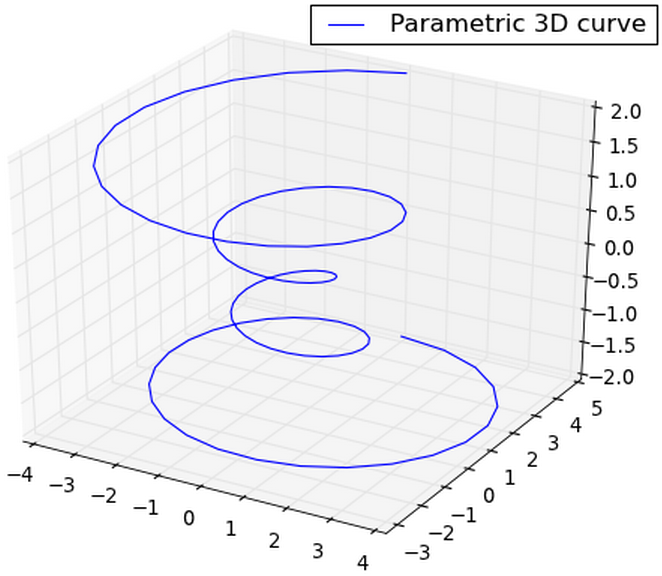
\includegraphics[width=0.6\textwidth]{imgp/plot3d-1.png}
\end{center}
\vspace{-4mm}
\caption{Plotting a parametric 3D curve.}
\label{fig:plot3d-1}
%\vspace{-1cm}
\end{figure}


\subsection{\ \ Plotting functions of two variables}

There are several ways to plot graphs of functions of two variables, 
first let us do this with Matplotlib's {\tt mplot3d} toolkit, then we will
use WebGL. We will plot the graph of the function 

$$
  f(x, y) = \sin(x) \sin(y)
$$
in the square $(-\pi, \pi) \times (-\pi, \pi)$.

\begin{verbatim}
# Import Numpy and Matplotlib:
from numpy import *
from mpl_toolkits.mplot3d import axes3d
import matplotlib.pyplot as plt

# Setup the 3D plot:
fig = plt.figure()
ax = fig.gca(projection='3d')

# Define intervals on the 'x' and 'y' axes and 
# their divisions (arange can be used as well):
x = linspace(-pi, pi, 30)
y = linspace(-pi, pi, 30)

# Create Cartesian grid:
X, Y = meshgrid(x, y)

# Calculate values at grid points:
Z = sin(X) * sin(Y)

# Plot the data:
ax.plot_wireframe(X, Y, Z, rstride=1, cstride=1)

# Show the plot:
lab.show()
\end{verbatim}
The parameters {\tt rstride} (row stride) and {\tt cstride} (column stride)
can be used to make the plot coarser when they are set to 2, 3, etc.
The output is shown in Fig. \ref{fig:plot3d-2}.
\newpage

\begin{figure}[!ht]
\begin{center}
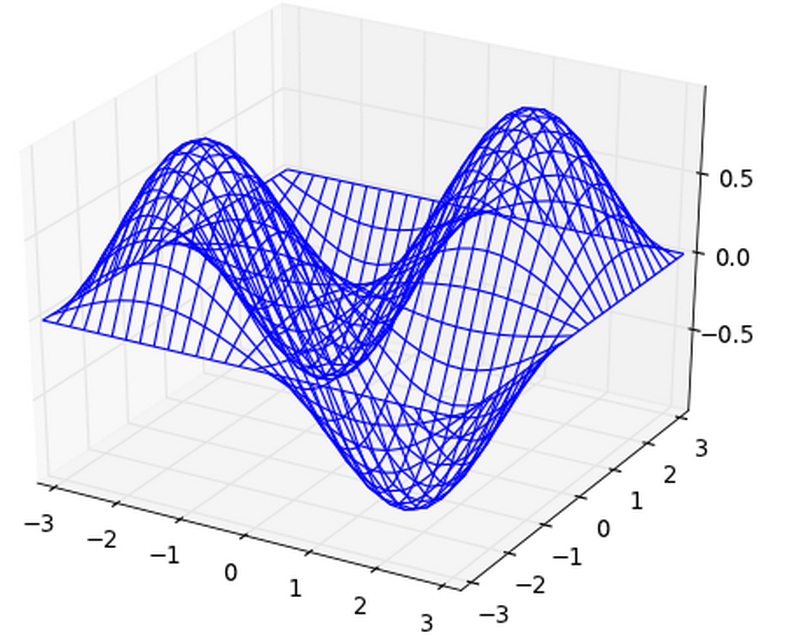
\includegraphics[width=0.6\textwidth]{imgp/plot3d-2.png}
\end{center}
\vspace{-4mm}
\caption{Wireframe plot of the function $f(x, y)$.}
\label{fig:plot3d-2}
%\vspace{-1cm}
\end{figure}
\noindent
Solid surface plot can be obtained by replacing in the above code 
{\tt plot\_wireframe} with {\tt plot\_surface}. 
The output is shown in Fig. \ref{fig:plot3d-3}.

\begin{figure}[!ht]
\begin{center}
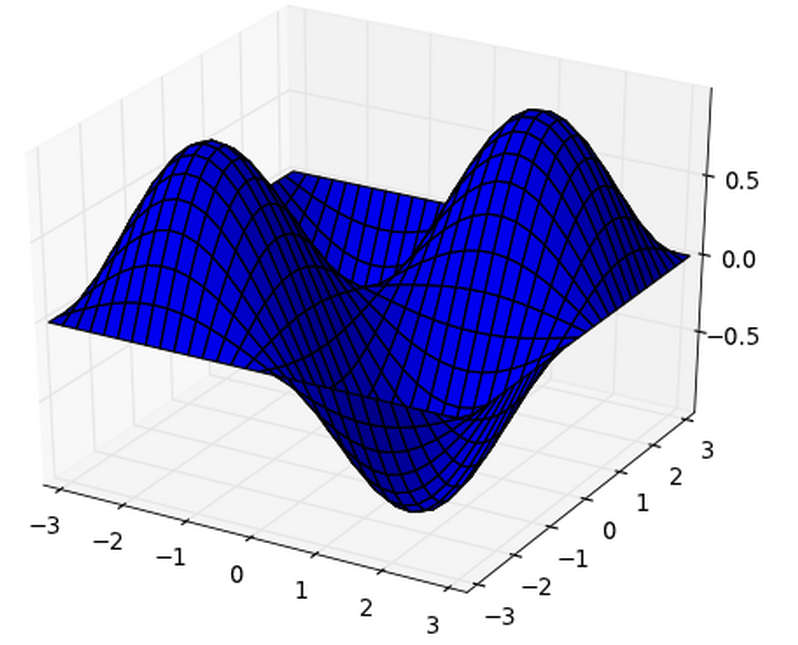
\includegraphics[width=0.6\textwidth]{imgp/plot3d-3.png}
\end{center}
\vspace{-4mm}
\caption{Surface plot of the function $f(x, y)$.}
\label{fig:plot3d-3}
%\vspace{-1cm}
\end{figure}
\newpage

\noindent
Contour plot can be obtained by replacing in the above code 
the line 

\begin{verbatim}
ax.plot_wireframe(X, Y, Z, rstride=1, cstride=1)
\end{verbatim}
with 

\begin{verbatim}
cset = ax.contour(X, Y, Z)
ax.clabel(cset)
\end{verbatim}
The output is shown in Fig. \ref{fig:plot3d-4}.

\begin{figure}[!ht]
\begin{center}
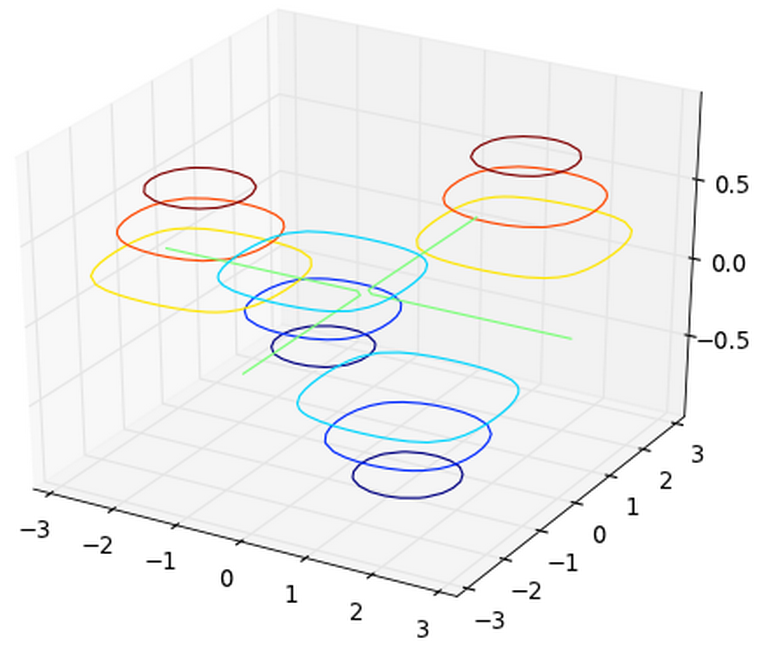
\includegraphics[width=0.6\textwidth]{imgp/plot3d-4.png}
\end{center}
\vspace{-4mm}
\caption{Contour plot of the function $f(x, y)$.}
\label{fig:plot3d-4}
%\vspace{-1cm}
\end{figure}
\noindent
We have only mentioned the most basic Matplotlib's functionality, for more options 
we refer to the tutorial 
at {\tt http://matplotlib.sourceforge.net/mpl\_toolkits/mplot3d}.


\subsection{\ \ Plotting functions of two variables with WebGL}

For this functionality, your browser has to support WebGL (most of modern browsers do, 
with the exception of Internet Explorer). See the introductory tutorial {\em Welcome to NCLab}
on the page {\tt http://femhub.com/nclab-tutorials/} for detailed instructions on how to enable WebGL. 
In the following example, we plot the graph of the function 

$$
  f(x, y) = \sin(\sqrt{x^2 + y^2})
$$
in the square $(0, 10) \times (0, 10)$.

\begin{verbatim}
from numpy import sin, sqrt, arctan

# Define intervals on the x and y axes.
x0 = 0.0
x1 = 10.0
y0 = 0.0
y1 = 10.0

# Define the corresponding divisions.
nx = 100
ny = 100

# Define the function:
def f(x, y):
    return sin(sqrt(x**2 + y**2))

# Render the surface using WebGL.
lab.surface((x0, x1, nx), (y0, y1, ny), f)
\end{verbatim}
The output is shown in Fig. \ref{fig:webgl}.

\begin{figure}[!ht]
\begin{center}
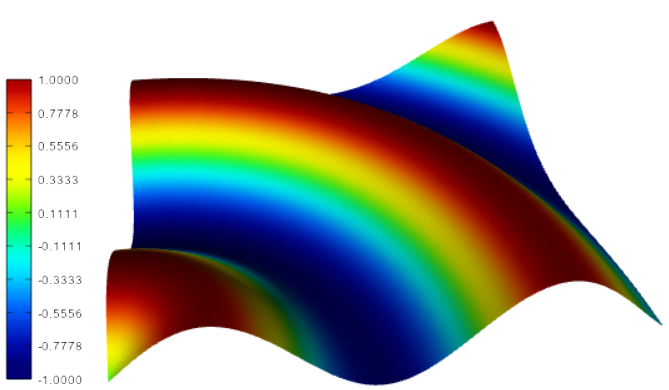
\includegraphics[width=0.6\textwidth]{imgp/webgl.png}
\end{center}
\vspace{-2mm}
\caption{Plotting functions of two variables with WebGL.}
\label{fig:webgl}
%\vspace{-1cm}
\end{figure}

\subsection{\ \ Review questions}

\begin{enumerate}
\item What is the result of $11 / 4$ in Python?
\begin{enumerate}
\item[A1] {\tt 2.75}
\item[A2] {\tt 2}
\item[A3] {\tt 3}
\item[A4] Error message is thrown.
\end{enumerate}
\item Type $3^2$ using Python syntax:
\begin{enumerate}
\item[A1] {\tt 3\^{}2}
\item[A2] {\tt 3\^{}\^{}2}
\item[A3] {\tt 3*2}
\item[A4] {\tt 3**2}
\end{enumerate}
\item Type $5$ modulo $2$ using Python syntax:
\begin{enumerate}
\item[A1] {\tt 5 / 2}
\item[A2] {\tt 5 \% 2}
\item[A3] {\tt 5 \& 2}
\item[A4] {\tt 5 \&\& 2}
\end{enumerate}
\item What is the result of $1**4*2$ in Python?
\begin{enumerate}
\item[A1] {\tt 0}
\item[A2] {\tt 1}
\item[A3] {\tt 2}
\item[A4] {\tt 4}
\end{enumerate}
\item What do we need to type into an empty Python worksheet in order to evaluate sin($\pi/4$)?
\begin{enumerate}
\item[A1] 
\begin{verbatim}
from numpy import sin
sin(pi/4)
\end{verbatim}
\item[A2] 
\begin{verbatim}
from numpy import sin, pi
sin(pi/4)
\end{verbatim}
\item[A3] 
\begin{verbatim}
from trigonometry import *
sin(pi/4)
\end{verbatim}
\item[A4] 
\begin{verbatim}
from trigonometry import sin, pi
sin(pi/4)
\end{verbatim}
\end{enumerate}
\item Which of the following are correct ways to define a complex number?
\begin{enumerate}
\item[A1] {\tt 2 + 3j}
\item[A2] {\tt 2 + 3J}
\item[A3] {\tt 2 + 3*j}
\item[A4] {\tt 2 + 3*J}
\end{enumerate}
\item Which of the following codes will draw a square with vertices [0, 0], [1, 0], [1, 1], [0, 1]?
\begin{enumerate}
\item[A1] 
\begin{verbatim}
from pylab import *
x = [0.0, 1.0, 1.0, 0.0]
y = [0.0, 0.0, 1.0, 1.0]
clf()
plot(x, y)
lab.show()
\end{verbatim}
\item[A2] 
\begin{verbatim}
from pylab import *
x = [0.0, 0.0, 1.0, 1.0]
y = [0.0, 1.0, 1.0, 0.0]
clf()
plot(x, y)
lab.show()
\end{verbatim}
\item[A3] 
\begin{verbatim}
from pylab import *
x = [0.0, 1.0, 1.0, 0.0, 0.0]
y = [0.0, 0.0, 1.0, 1.0, 0.0]
clf()
plot(x, y)
lab.show()
\end{verbatim}
\item[A4] 
\begin{verbatim}
from pylab import *
x = [0.0, 0.0, 1.0, 1.0, 0.0]
y = [0.0, 1.0, 1.0, 0.0, 0.0]
clf()
plot(x, y)
lab.show()
\end{verbatim}
\end{enumerate}
\item Which of the following codes will plot a cosine function in the interval $(0, \pi)$ using dashed green line with
the step 0.01?
\begin{enumerate}
\item[A1] 
\begin{verbatim}
from numpy import cos, pi
from pylab import *
x = arange(0, pi, 0.01)
y = cos(x)
axis=("equal")
clf()
plot(x, y, 'g-', label="cos(x)")
legend()
lab.show()
\end{verbatim}
\item[A2] 
\begin{verbatim}
from numpy import cos, pi
from pylab import *
x = arange(0, pi, 0.01)
y = cos(x)
clf()
plot(x, y, 'g--')
lab.show()
\end{verbatim}
\item[A3] 
\begin{verbatim}
from numpy import cos, pi
from pylab import *
x = arange(0, pi, 0.01)
y = cos(x)
axis=("equal")
clf()
plot(x, y, 'g--', label="cos(x)")
legend()
lab.show()
\end{verbatim}
\item[A4] 
\begin{verbatim}
from numpy import cos, pi
from pylab import *
x = arange(0, pi, 0.01)
y = cos(x)
axis=("equal")
clf()
plot(x, y, 'g..', label="cos(x)")
legend()
lab.show()
\end{verbatim}
\end{enumerate}
\end{enumerate}

\subsection{\ \ Programming exercises}
Perform the following calculations using the Python worksheet.
\begin{enumerate}
\item 
$$
  987654321 - 123456789
$$
\item 
$$
\frac{8}{5}
$$
\item 
$$
  \frac{8237456 + 289374}{23784}
$$ 
\item 
$$
  3645^2
$$
\item 
$$
  318476256 \ \mbox{modulo} \ 7
$$
\item 
$$
  \frac{3\cdot 2^2}{5} 
$$
\item 
$$
  e^8
$$
\item 
$$
  \ln 4082374
$$
\item 
$$
  \sin(\pi / 4)
$$
\item 
$$
  (1 + 2i)(3 - i)
$$
where $i$ is the imaginary unit.
\item Write a Python program to plot a polygon with $N$ equally-long edges that is inscribed into a circle of 
center $[x_0, y_0]$ and radius $R > 0$. Here $N \ge 3$ is an integer number and $x_0, y_0, R$ are real numbers
The user should be able to change all of them. Axes should be scaled equally.
\item Write a Python program to plot a circle of center $[x_0, y_0]$ and radius $R > 0$, where 
$x_0, y_0$ and $R$ are variables that the user can change. Axes should be scaled equally.
\item Write a Python program to plot an ellipse with focal points $[x_0, 0]$ and $[-x_0, 0]$ where 
$x_0 > 0$ is a variable that the user can change. Axes should be scaled equally.
\item The function {\tt random()} returns a random number between $0$ and $1$ (it can be $0.0$ but it cannot be $1.0$).
Write a Python program to generate and plot a random triangle that lies in the unit square $[0, 1) \times [0, 1)$. 
\item Display wireframe plot of the function 
$$
f(x, y) = e^{-x^2 - y^2}
$$
in the square $(-3, 3)\times (-3, 3)$.
\item Display solid surface plot of the function 
$$
f(x, y) = 5 - \sqrt{x^2 + y^2}
$$
in the square $(-2, 2)\times (-2, 2)$.
\item Display contour plot of the function 
$$
f(x, y) = \sin(x) \cos(y) 
$$
in the square $(-2\pi, 2\pi)\times (-2\pi, 2\pi)$.
\item Display WebGL plot of the function
$$
f(x, y) = e^{-x^2 - y^2}
$$
in the square $(-1, 1)\times (-1, 1)$.

\end{enumerate}

\section{Functions}

\subsection{Objectives}

\begin{itemize}
\item Learn to define custom functions in Python.
\item Learn to use default arguments and return multiple values.
\end{itemize}
Custom {\em functions} in Python are the same thing as custom procedures in Karel,
but in Python they can moreover {\em accept arguments}. Recall that new procedures in Karel were 
defined to make some functionality easily reusable -- functions in Python are defined for the same reason.

\subsection{Defining new functions}

Definition of a new function begins with the keyword {\tt def} as in Karel. In Python,
we moreover use round brackets for arguments and a colon at the end of the line. 
For example, the following function adds two numbers
and returns the result:

\begin{verbatim}
def add(a, b):
    return a + b
\end{verbatim}
The round brackets in the function definition are mandatory even if no arguments are passed,
and the {\tt return} statement can be omitted if not needed.
The two lines of code above 
are a {\em function declaration} -- they do not produce any output.
In order to call the function, we need to write one additional line, such as:

\begin{verbatim}
print "5 + 3 is", add(5, 3)
\end{verbatim}
This will produce the following output:

\begin{verbatim}
5 + 3 is 8
\end{verbatim}
To show another example, the following function does not take any arguments 
and it does not return any results:

\begin{verbatim}
def hello():
    print "Hello!"
\end{verbatim}

\subsection{Passing arbitrary arguments}

Python does not require that we specify the type of function arguments. 
What does it mean? The above function {\tt add(a, b)} works for real
numbers, complex numbers, vectors, strings, and any other 
objects where the operation '+' is defined. Let's try this:

\begin{verbatim}
def add(a, b):
    return a + b

word1 = "Good "
word2 = "Evening!"
print add(word1, word2)
\end{verbatim}
Output:

\begin{verbatim}
Good Evening!
\end{verbatim}
Things like this make Python very intuitive and easy to use. In conventional languages such as C or C++, 
we would have to define different functions: {\tt add\_real\_numbers(a, b)} for real numbers,
{\tt add\_complex\_numbers(a, b)} for complex numbers numbers, {\tt add\_strings(a, b)} for strings, etc. 
In C, they would be as follows:

\begin{verbatim}
double add_real_numbers(double a, double b)
{
  return a + b;
}
\end{verbatim}
and

\begin{verbatim}
# include <complex.h>
complex add_complex_numbers(complex a, complex b)
{
  return a + b;
}
\end{verbatim}
and 

\begin{verbatim}
void add_strings(const char* a_in, const char* b_in, char* c_out)
{
  strcpy(c_out, a_in);
  strcat(c_out, b_in);
  return;
}
\end{verbatim}

\subsection{Returning multiple values}

Python functions can return multiple values which often comes handy.
For example, the following function returns the 
second, third, and fourth powers of a number:

\begin{verbatim}
def powers(a):
    return a**2, a**3, a**4
\end{verbatim}
This is how the function is used:

\begin{verbatim}
var1 = 2
print "Powers are", powers(var1)
\end{verbatim}
Output:

\begin{verbatim}
Powers are (4, 8, 16)
\end{verbatim}
We can also store the returned values in three separate variables:

\begin{verbatim}
var1 = 3
p2, p3, p4 = powers(var1)
print "Powers are", p2, p3, p4
\end{verbatim}
Output:

\begin{verbatim}
Powers are 9 27 81
\end{verbatim}
Look how complicated the same program would be in C/C++:

\begin{verbatim}
void powers(double a, double* p2, double* p2, double* p3)
{
  *p2 = pow(a, 2);
  *p3 = pow(a, 3);
  *p4 = pow(a, 4);
  return;
}

int main()
{
  double p1, p2, p3;
  double a = 2;
  powers(a, &p2, &p2, &p3);
  printf("Powers are %g, %g, %g.\n", p2, p3, p4);
}
\end{verbatim}

\subsection{Using default arguments}

Holland is the most bicycle friendly country in the world. Imagine that you 
work for the Holland Census Bureau. Your task is to ask 10000 
people how they go to work, and enter their answers into a database. 
The program for entering data into the database was written by one of 
your colleagues, and it can be used as follows:

\begin{verbatim}
add_database_entry("John", "Smith", "walks")
\end{verbatim}
or 
\begin{verbatim}
add_database_entry("Louis", "Armstrong", "bicycle")
\end{verbatim}
or
\begin{verbatim}
add_database_entry("Jim", "Bridger", "horse")
\end{verbatim}
etc. Since you are in Holland, it can be expected that $99 \%$ of people 
are using the bicycle. In principle you could call the function {\tt add\_database\_entry()} 
to enter each answer, but with 9900 bicyclists out of 10000 respondents you would have to 
type {\tt "bicycle"} MANY times. 

Fortunately, Python offers a smarter way to do this. We can define a new function 

\begin{verbatim}
def enter(first, last, transport = "bicycle"):
    enter_into_database(first, last, transport)
\end{verbatim}
This is a simple ({\em "thin"}) {\em wrapper} to the function {\tt add\_database\_entry()} 
that allows us to omit the third argument in the function call and autocomplete 
it with a {\em default argument} {\tt "bicycle"}. In other words, now we do not have to 
type {\tt "bicycle"} for Louis Armstrong or any other bicyclist:

\begin{verbatim}
enter("Louis", "Armstrong")
\end{verbatim}
Only if we meet a rare someone who uses a car, we type 

\begin{verbatim}
enter("Niki", "Lauda", "car")
\end{verbatim}
Another example: Let us return to the function {\tt add()}, and let us 
imagine that very often (but not always) the second number that we
are adding is 10. Then it makes sense to write the function {\tt add()}
as follows:

\begin{verbatim}
def add(a, b = 10):
    return a + b
\end{verbatim}
The function will work as before when called with two arguments: 

\begin{verbatim}
A = 5
B = 1
add(A, B)
\end{verbatim}
Output:
\begin{verbatim}
6
\end{verbatim}
But it can be also called with the second argument omitted:
\begin{verbatim}
A = 5
add(A)
\end{verbatim}
Output:
\begin{verbatim}
15
\end{verbatim}
\underline{Some rules to remember}:
\begin{itemize}
\item Default arguments need to be introduced {\bf after} standard (non-default) arguments. In other words, the 
      following code will result into an error:
\begin{verbatim}
def add(a = 5, b):
    return a + b
\end{verbatim}
This is the error message:
\begin{verbatim}
  File "<nclab>", line 1
SyntaxError: non-default argument follows default argument

\end{verbatim}
\item If multiple default arguments are present, they have to follow the non-default ones.
      If the number of arguments in the function call is less than the total number of default and non-default
      arguments, then first all non-default arguments are assigned, and then the default ones from 
      left to right. To illustrate this, assume the function:
\begin{verbatim}
def add(x, a = 2, b = 3):
    return x + a + b
\end{verbatim}
This function can be called as follows:
\begin{verbatim}
print add(1)
\end{verbatim}
In this case, the value {\tt 1} is assigned to {\tt x} and {\tt a} and {\tt b} take the default values.
The output will be 
\begin{verbatim}
6
\end{verbatim}
When the function is called with just two values,
\begin{verbatim}
print add(5, 6)
\end{verbatim}
then the value {\tt 5} is assigned to {\tt x}, {\tt 6} to {\tt a}, and {\tt b} takes the default value {\tt 3}.
The output is
\begin{verbatim}
14
\end{verbatim}
However, it is always a good idea to be as transparent as possible. Therefore a better code is 
\begin{verbatim}
print add(1, a = 6)
\end{verbatim}
Then the result is the same, {\tt 14}, but it is clear even to non-experts what is going on. Moreover,
in this way we can also define the value of {\tt b} without having to define the value of {\tt a}:
\begin{verbatim}
print add(1, b = 6)
\end{verbatim}
Now {\tt x} is {\tt 1}, {\tt a} has the default value {\tt 2} and the result is {\tt 9}.
\end{itemize}

\subsection{Review questions}

\begin{enumerate}
\item Why do we define {\em functions} in programming? 
\begin{enumerate}
\item[A1] To isolate self-contained functionality and make it easily reusable.
\item[A2] To make computer programs faster.
\item[A3] To split long programs into multiple segments that have fewer lines.
\item[A4] We should not use functions, it is not a good programming practice.
\end{enumerate}
\item Which of the following are correct function definitions?
\begin{enumerate}
\item[A1] 
\begin{verbatim}
def subtract(a, b)
    return a - b
\end{verbatim}
\item[A2] 
\begin{verbatim}
def subtract(a, b):
    return a - b
\end{verbatim}
\item[A3] 
\begin{verbatim}
def subtract[a, b]
    return a - b
\end{verbatim}
\item[A4] 
\begin{verbatim}
def subtract(a, b = 5):
    return a - b
\end{verbatim}
\end{enumerate}
\item When do we have to specify argument types in Python functions?
\begin{enumerate}
\item[A1] Never.
\item[A2] Always.
\item[A3] Always except for numbers and text strings.
\item[A4] Only when default arguments are used.
\end{enumerate}
\item We know from Section \ref{sec:calc} that the modulo operation calculates the 
      rest after integer division. Assume positive integers $a > 0$ and $b > 0$.
      The number $a$ can be decomposed as follows:
      $$
      a = nb + r
      $$  
      where $n \ge 0$ and $0 \le r < b$ are integers.
      Which of the following functions will do the job
      and return the numbers {\tt n} and {\tt r} ?
\begin{enumerate}
\item[A1] 
\begin{verbatim}
def splitnumber(a, b)
    return a / b, a % b
\end{verbatim}
\item[A2] 
\begin{verbatim}
def splitnumber(a, b)
    return a % b, a / b
\end{verbatim}
\item[A3] 
\begin{verbatim}
def splitnumber(a, b):
    n = a / b
    r = a % b
    return n
    return r
\end{verbatim}
\item[A4] 
\begin{verbatim}
def splitnumber(a, b):
    return a / b, a % b
\end{verbatim}
\end{enumerate}
\item Of the following four functions, choose the best one to calculate the hypotenuse
      of a right-angled triangle when you know that most of the time one of its shorter
      edges will be 5 cm long?
\begin{enumerate}
\item[A1] 
\begin{verbatim}
from numpy import sqrt
def hypotenuse(a, b):
    return sqrt(a**2 + b**2)
\end{verbatim}
\item[A2] 
\begin{verbatim}
from numpy import sqrt
def hypotenuse(a = 5, b):
    return sqrt(a**2 + b**2)
\end{verbatim}
\item[A3] 
\begin{verbatim}
from numpy import sqrt
def hypotenuse(a, b = 5):
    return sqrt(a**2 + b**2)
\end{verbatim}
\item[A4] 
\begin{verbatim}
from numpy import sqrt
def hypotenuse(a = 5, b = 5):
    return sqrt(a**2 + b**2)
\end{verbatim}
\end{enumerate}
\end{enumerate}

\subsection{Programming exercises}

\begin{enumerate}
\item Write a Python function {\tt circle} that accept an arbitrary positive radius $R > 0$
      as argument, and returns the area and the perimeter of a circle with radius $R$.
\item Write a Python function {\tt squarearea} that returns the area of a square whose 
      edge is $a$ cm long. You know that most of the time the edge length wil be 1 cm,
      so make this function callable without any arguments.
\item Write a Python function {\tt rectanglearea} that returns the area of a rectangle 
      whose edges are $a$ and $b$ cm long. You know that most of the time one of the edges 
      will measure 3 cm, so make the function callable with only one argument.
\end{enumerate}

\section{More on Variables}

\subsection{Objectives}

\begin{itemize}
\item Understand dynamic type interpretation.
\item Learn about {\em local} and {\em global} variables.
\item Understand why global variables should be avoided.
\item Learn about {\em variable shadowing}.
\end{itemize}
The reason why we use variables is the same in Karel the Robot, Python, and all other programming 
languages -- to store useful information for later use. Also the way we work with variables is almost the 
same, so we will just mention a few aspects that are new in Python.

\subsection{Assigning values to variables}

In Python, several variables can be initialized at the same time:

\begin{verbatim}
x = y = z = 0.0
print "x =", x
print "y =", y
print "z =", z
\end{verbatim}
Output:

\begin{verbatim}
x = 0.0
y = 0.0
z = 0.0
\end{verbatim}
As in Karel, variables must be defined (have a value assigned) before they can be 
used. 

\subsection{Dynamic type interpretation}

Python is very generous with the types of variables -- it will figure out the type of a variable 
at runtime, depending on the value that we store in it. The type can even change at runtime.
For example, let us look at the following code:

\begin{verbatim}
a = 5
print a
a = "Hi!"
print a
a = True
print a
\end{verbatim}
The output is 

\begin{verbatim}
5
Hi!
True
\end{verbatim}
This is very different from compiled languages such as C, C++ where one needs to declare the type 
of every variable before its first use, and the type then cannot be changed. 

\subsection{Changing values of variables}

The simplest way to increase the value of a numerical variable in Python by a given number 
is to use the '{\tt +=}' command:

\begin{verbatim}
v = 1
v += 3
print "v =", v
\end{verbatim}
Output:

\begin{verbatim}
v = 4
\end{verbatim}
We can also subtract a number from a numerical variable:

\begin{verbatim}
v -= 1
print "New value of v is", v
\end{verbatim}
Output:

\begin{verbatim}
New value of v is 3
\end{verbatim}
We can multiply a numerical variable with a number:

\begin{verbatim}
v *= 4
print "Now v is", v
\end{verbatim}
Output:

\begin{verbatim}
Now v is 12
\end{verbatim}
And finally, we can divide a numerical variable with a number:

\begin{verbatim}
v /= 6
print "Finally, v is", v
\end{verbatim}
Output:

\begin{verbatim}
Finally, v is 2
\end{verbatim}
It is possible to use existing variables to assign a value to a new variable:

\begin{verbatim}
a = 1
b = 2.5
c = 0.5
d = (a + b) / c
print "d =", d
\end{verbatim}
Output:

\begin{verbatim}
d = 7.0
\end{verbatim}
Of course, apples cannot be mixed with oranges. When we try to 
add a number to a text string,

\begin{verbatim}
a = "My car is a Ferrari."
b = 3.5

c = a + b
\end{verbatim}
then the interpreter rightfully complains:

\begin{verbatim}
Traceback (most recent call last):
  File "<nclab>", line 4, in <module>
TypeError: cannot concatenate 'str' and 'float' objects
\end{verbatim}

\subsection{Local and global variables}

If a variable was defined inside of a function, then it is {\em local} to that
function. Imagine a lake -- a fish born in a lake will always 
stay in that lake (fishing neglected). If we try to access 
the variable outside that function, even though the function was 
already called, the variable will be unknown. Look at the following 
code:

\begin{verbatim}
def add(a, b):
    c = a + b
    return c

print "Sum of 3 and 4 is", add(3, 4)
print c
\end{verbatim}
The output is:

\begin{verbatim}
Sum of 3 and 4 is 7
Traceback (most recent call last):
  File "<nclab>", line 6, in <module>
NameError: name 'c' is not defined
\end{verbatim}
In computer programming, {\em we want all our variables to be local}, because 
this avoids name clashes and minimizes the risk of unwanted side effects.
Mistakes such as unwanted overwriting of the value stored in a global variable 
belong to the worst to deal with.

\subsection{Sure method to spoil your code}

Once a variable is used in the main program, 
then it is {\em global}, meaning that you could use it in 
any function that you define. Like in the following 
code:

\begin{verbatim}
val = 5.0

def msg():
    print "val =", val

msg()
\end{verbatim}
Brrr, this code is ugly! But it works (unfortunately), see the output:

\begin{verbatim}
val = 5.0
\end{verbatim}
Remember:\\

\begin{center}
{\em Passing global variables to functions is a bad habit that makes your code\\
     difficult to understand, prone to mistakes, and extremely difficult to fix}.\\
\end{center}
\vspace{4mm}
\noindent
A function should always
obtain all the data it needs through its arguments. Imagine that a unit of soldiers 
would act based not only on orders it receives (that's the argument 
list), but also based on rumors that some of the soldiers read in a Sunday magazine. 
That might not work well!\\

\noindent
A clean version of the above code is

\begin{verbatim}
def msg(v):
    print "val =", v

val = 5.0

msg(val)
\end{verbatim}
Can you see the difference? Now the function {\tt msg} is {\em readable} -- you do not 
need to look elsewhere in the program to understand what it does. The output is:

\begin{verbatim}
val = 5.0
\end{verbatim}

\subsection{Variable shadowing}

Sometimes, by accident or intentionally, we may have two different 
variables of the same name in the code. Look, for example, at this short program:

\begin{verbatim}
c = 5

def add(a, b):
    c = a + b
    print "c =", c
    return c

add(1, 2)
print "c =", c
\end{verbatim}
The output is

\begin{verbatim}
c = 3
c = 5
\end{verbatim}
There is no 
problem with the last line of the program because the local variable {\tt c}, defined
inside of the function {\tt add}, is no longer defined there. But inside of the function
{\tt add}, both the global variable {\tt c} and the local variable {\tt c} are defined at 
the same time. This is commonly referred to as {\em variable shadowing}, and we need to 
remember that if this happens, {\bf the local variable is used}.

\subsection{Review questions}

\begin{enumerate}
\item Which of the following code(s) is/are invalid in Python?
\begin{enumerate}
\item[A1] 
\begin{verbatim}
a = b = 1
\end{verbatim}
\item[A2] 
\begin{verbatim}
a = 1 = b
\end{verbatim}
\item[A3] 
\begin{verbatim}
a = a
\end{verbatim}
\item[A4] 
\begin{verbatim}
a + b = 5
\end{verbatim}
\end{enumerate}
\item When can a given variable have different types in a Python program?
\begin{enumerate}
\item[A1] Any time.
\item[A2] Never.
\item[A3] Only when variable shadowing takes place.
\item[A4] Only when the types are real number and integer number.
\end{enumerate}
\item We have two variables {\tt a} and {\tt b} and need to swap their values. Which of the 
following codes will do it?
\begin{enumerate}
\item[A1] 
\begin{verbatim}
a = b = a
\end{verbatim}
\item[A2] 
\begin{verbatim}
a = b
b = a
\end{verbatim}
\item[A3] 
\begin{verbatim}
a = b
c = a
b = a
\end{verbatim}
\item[A4] 
\begin{verbatim}
c = a
a = b
b = c
\end{verbatim}
\end{enumerate}
\item Should we preferably use local variables, or global variables, and why?
\begin{enumerate}
\item[A1] Global variables because they can be all defined in one place.
\item[A2] Global variables because it yields a faster code.
\item[A3] Local variables because then we can use shadowing.
\item[A4] Local variables because our code is less prone to mistakes. 
\end{enumerate}
\item Should we use global variables in functions and why?
\begin{enumerate}
\item[A1] Yes, the function definition is simpler.
\item[A2] Yes, the program is less prone to mistakes.
\item[A3] No, it makes the code less transparent and more prone to mistakes.
\item[A4] No, Python does not allow it.
\end{enumerate}
\item What is variable shadowing?
\begin{enumerate}
\item[A1] There are two or more functions that all use a local variable of the same name.
\item[A2] The type of a global variable is changed by assigning value of a different type to it. 
\item[A3] The type of a local variable is changed by assigning value of a different type to it. 
\item[A4] There is a local variable whose name matches the name of a global one.
\end{enumerate}
\end{enumerate}

\subsection{Programming exercises}

\begin{enumerate}
\item The number $\pi$ can be written as an infinite series 
$$
\pi = 4\left(1 - \frac{1}{3} + \frac{1}{5} - \frac{1}{7} + \frac{1}{9} - \ldots     \right).
$$
Write a Python function {\tt approx\_pi()} that returns an approximation of $\pi$ using a truncated 
series where the last fraction used is $1/13$.
\item {\em Arithmetic sequence} is a progression of $n$ numbers $a_1$, $a_2$, $\ldots$, $a_n$
that increase by the same difference $d$. For example, 
$$
5, 7, 9, 11, 13, 15, 17
$$
is an arithmetic sequence with $n = 7$, $a_1 = 5$ and $d = 2$. It holds
$$
a_n = a_1 + (n-1)d.
$$
There is a well known formula for the sum of such a sequence:
$$
S = \frac{n}{2}(a_1 + a_n).
$$
And now the exercise: Write a function {\tt summation\_arithmetic(n, a1, d)} that takes arbitrary 
values of $n$, $a_1$ and $d$ as arguments, and calculates and returns the sum
of the corresponding arithmetic sequence! 
\item {\em Geometric sequence} is a progression of $n$ numbers $a_1$, $a_2$, $\ldots$, $a_n$
where the next number is calculated by multiplying the last one with a quotient $q$.
For example, 
$$
1, \frac{1}{2}, \frac{1}{4}, \frac{1}{8}, \frac{1}{16}
$$
is a geometric sequence with $n = 5$, $a_1 = 1$ and $q = 1/2$. It is 
$$
a_n = a_1 \cdot q^{n-1}.
$$
If $q \not = 1$, then the formula for the sum of such a sequence is
$$
S = a_1\frac{1 - q^n}{1 - q}
$$
Write a function {\tt summation\_geometric(n, a1, q)} that takes arbitrary 
values of $n$, $a_1$ and $q \not = 1$ as arguments, and calculates 
and returns the sum of the corresponding geometric sequence! 
\item {\em Sales prediction}. The East Coast sales division of a company usually generates $P$
percent of total sales each year. Write a function {\tt sales\_prediction(P, S)} to predict how much 
the East Coast division will generate if the company has $S$ dollars in sales the next year. 
Use your function with the numbers $P = 62\ \%$ and $S = 4.6$ million dollars. 
\item {\em Sales tax}. 
Write a function {\tt sales\_tax(P, ST, CT)} that calculates the total sales tax on a $P$ dollars purchase. 
Assume the state sales tax is $ST$ percent, and the county sales tax is $CT$ percent. Use the
function with the following numbers: $P = 52$ dollars, $ST = 5 \%$, $CT = 2 \ \%$.
\item {\em Restaurant bill}. Write a function {\tt restaurant\_bill(M, P, T)} 
that computes the tax and tip on a restaurant bill for a patron with 
$M$ dollars meal charge. The tax is $P$ percent of the meal cost. The tip is $T$ percent of the total after 
adding the tax. Your function should print the meal cost, 
tax amount, and tip amount, and return the total bill. Use your function with 
the numbers $M = 44.50$ dollars, $P = 6.75 \ \%$ and $T = 15 \ \%$. 
\item {\em Gas consumption I}. In Europe, gas consumption of a car is reported in liters per 100 kilometers. In the U.S. 
it is reported in miles per gallon. Write a function {\tt conversion\_eu\_to\_us(C)} that converts a given European 
gas consumption $C$ into the U.S. scale. One mile is 1.6 kilometers, and one gallon is 3.78541178 liters. 
\item {\em Gas consumption II}. Write a function {\tt conversion\_us\_to\_eu(C)} that converts a given U.S.
gas consumption $C$ into the European scale.
\item {\em Distance per tank of gas}. A car with a $G$ gallon gas tank averages $A$ miles per gallon 
when driven in town and 
$B$ miles per gallon when driven on the highway. Write a function {\tt distance(G, A, B)} 
that calculates and prints 
the distance the car can travel on one tank of gas when driven in town and when driven on the highway. 
Use your function with $G = 20$ gallons, $A = 21.5$ miles per gallon, $B = 26.8$ miles per gallon. 
\item {\em Circuit board price.} An electronics company sells circuit boards at a $P$ percent profit. 
Write a function {\tt circuit\_board\_price(P, D)} 
that calculates the selling price of a circuit board that costs them $D$ dollars to
produce. Use your function with $P = 40\ \%$ and $D = 12.67$ dollars.
\item {\em Gross pay}. A particular employee earns $E$ dollars annually. Write a function 
{\tt gross\_pay(E)} that determines and prints what the amount of his gross pay will be for each pay period 
if he is paid twice a month (24 pay checks per year) and if he is paid bi-weekly (26 checks per 
year). Use your function with $E = 32,500$ dollars.
\item {\em Stock gain}. Kathryn bought $600$ shares of stock at a price of $A$ dollars per share. 
One year later she 
sold them for $B$ dollars per share. Write a function {\tt stock\_gain(A, B)} that calculates and 
displays the following:
\begin{itemize}
\item The total amount paid for the stock.
\item The total amount received from selling the stock.
\item The total amount of money she gained.
\end{itemize}
Use your function with the values $A = 21.77$ dollars and $B = 26.44$ dollars.
\end{enumerate}

\section{Review of Logic}

\subsection{Objectives}

\begin{itemize}
\item Review Boolean expressions, operations, and variables.
\end{itemize}
There are virtually no changes compared to Karel the Robot, so we will 
only revisit the subject briefly. 

\subsection{Boolean expressions}

Let's begin with creating a variable 
and printing it:

\begin{verbatim}
a = 1
print a
\end{verbatim}
Output:

\begin{verbatim}
1
\end{verbatim}
Now type

\begin{verbatim}
print a > 0
\end{verbatim}
Output:

\begin{verbatim}
True
\end{verbatim}
Although the syntax looks a bit unusual, this is a correct
Python code -- since {\tt a} is one, the Boolean expression {\tt a > 0}
is {\tt True}. This is the value that gets printed. We can try it the other 
way round:

\begin{verbatim}
print a < 0
\end{verbatim}
Output:

\begin{verbatim}
False
\end{verbatim}

\subsection{Boolean variables}

We can also store the value of the expression {\tt a > 0} in a Boolean variable,
and print it:
\begin{verbatim}
b = a < 0
print b
\end{verbatim}
Output:

\begin{verbatim}
False
\end{verbatim}
Boolean expressions involving numbers often contain the following operators:

\begin{center}
\begin{tabular}{|c|l|}
\hline
Symbol & Meaning \\
\hline
{\tt >} & greater than\\
{\tt >=} & greater than or equal to\\
{\tt <=} & less than or equal to\\
{\tt <} & less than\\
{\tt ==} & equal to\\
{\tt !=} & not equal to\\
{\tt <>} & not equal to (same as {\tt !=})\\
\hline
\end{tabular}
\end{center}

\subsection{Boolean operations}

With Boolean variables we can do logical operations such as {\tt and}:

\begin{verbatim}
a = 1
v1 = a > 0
v2 = a < 5
print v1 and v2
\end{verbatim}
Output:

\begin{verbatim}
True
\end{verbatim}
Logical {\tt or}:

\begin{verbatim}
v3 = a > 10
print v1 or v3
\end{verbatim}
Output:

\begin{verbatim}
True
\end{verbatim}
Negation:

\begin{verbatim}
v4 = not v1
print v4
\end{verbatim}
Output:

\begin{verbatim}
False
\end{verbatim}
Sometimes logical expressions can be more complicated, but this is no problem
as we always can use round brackets: 

\begin{verbatim}
v5 = not ((v1 and v2) or (v3 and not v4))
\end{verbatim}

\subsection{Review questions}

\begin{enumerate}
\item Let {\tt a} and {\tt b} be Boolean variables. What is the 
result of {\tt (a or b) or (not (a or b))}
\begin{enumerate}
\item[A1] {\tt False}
\item[A2] Undefined.
\item[A3] {\tt False} or {\tt True}, depending on the values of {\tt a} and {\tt b}.
\item[A4] {\tt True}
\end{enumerate}
\item Let {\tt a} and {\tt b} be Boolean variables. What is the 
result of {\tt (a and b) and (not (a and b))}
\begin{enumerate}
\item[A1] Undefined.
\item[A2] {\tt False} or {\tt True}, depending on the values of {\tt a} and {\tt b}.
\item[A3] {\tt True}
\item[A4] {\tt False}
\end{enumerate}
\end{enumerate}


\subsection{Programming exercises}

\begin{enumerate}
\item Write a Python function {\tt checknumber(n)} where {\tt n} is an arbitrary 
      integer number, that returns {\tt True} if {\tt n} is even and {\tt False}
      otherwise.
\item Consider a quadratic equation $ax^2 + bx + c = 0$ where $a, b, c$ are real numbers 
      and $a \not = 0$. Write a Python function 
      {\tt hasrealroots(a, b, c)} that returns {\tt True} if the equation has 
      at least one real root, and {\tt False} otherwise.
\item Write a Python function {\tt liesincircle(R, x, y)} that returns {\tt True} if 
      the point with planar coordinates {\tt [x, y]} lies in a circle of radius {\tt R}
      whose center is at the origin {\tt [0, 0]}. If the point lies on the border of the 
      circle or outside, the function should return {\tt False}.
\end{enumerate}

\section{More on Conditions}

\subsection{Objectives}

\begin{itemize}
\item Review and refine your knowledge of conditions.
\item Learn to always perform sanity checks of user input.
\end{itemize}
Each procedural programming language including Python enables conditional 
execution of code. What does this mean? Imagine that you have to write
a program to calculate
$$
\frac{1}{9 - x^2}
$$
for any value of $x$. Of course, this is simple:

\begin{verbatim}
result = 1. / (9 - x**2)
print "Result is", result
\end{verbatim}
However, when a user calls your program with $x = 3$ or $x = -3$, then
it crashes!

\begin{verbatim}
Traceback (most recent call last):
  File "<nclab>", line 1, in <module>
ZeroDivisionError: float division by zero
\end{verbatim}
This is not a good thing to happen, and thus we need to be more careful.
Here is an alternative version of the program that will not crash:

\begin{verbatim}
if (x == 3) or (x == -3):
    print "Result is undefined, division by zero!"
    result_defined = False
else:
    result = 1. / (9 - x**2)
    print "Result is", result
    result_defined = True
\end{verbatim}
Notice that the lines in the {\tt if} and {\tt else} branches are indented,
The indent means that a command is still inside the {\tt if} or {\tt else}
branch.

Failure to use indents properly will result into an incorrect program. For 
example, if we forgot to indent the last line in the above program,

\begin{verbatim}
if (x == 3) or (x == -3):
    print "Result is undefined, division by zero!"
    result_defined = False
else:
    result = 1. / (9 - x**2)
    print "1 / (9 - x**2) =", result
result_defined = True
\end{verbatim}
then the last line would be outside of the {\tt if - else} statement, and
thus the variable {\tt result\_ defined} would be always {\tt True}!\\

\noindent
Sometimes the {\tt else} branch is not needed, and in that case it can be omitted:

\begin{verbatim}
if (x != 3) and (x != -3):
    result = 1. / (9 - x**2)
    print "Result is", result
    result_defined = True
\end{verbatim}
Sometimes we need to consider more cases. For this, we can use {\tt elif}
(abbreviation for "else if"):

\begin{verbatim}
if (x == 3) or (x == -3):
    print "Result is undefined, division by zero!"
elif abs(x) < 3:
    print "Result is positive."
else:
    print "Result is negative."
\end{verbatim}
There can be more {\tt elif} statements if needed. \\

\noindent
In more complicated cases, conditions can be embedded in other conditions:

\begin{verbatim}
if (x == 3) or (x == -3):
    print "Result is undefined, division by zero!"
elif abs(x) < 3:
    if x < 0:
        print "x is negative and result is positive."
    else: 
        print "x is positive and result is positive."
else:
    if x < 0:
        print "x is negative and result is negative."
    else: 
        print "x is positive and result is negative."
\end{verbatim}
If your head hurts, do not worry. This section is over 
and the next one is going to be simpler!

\subsection{Review questions}

\subsection{Programming exercises}


\section{More on the {\tt while} loop}\label{sec:while}

\subsection{Objectives}

\begin{itemize}
\item
\end{itemize}

Loops are a powerful tool as they allow us to use the computer to solve
tasks that would take many hours, months, or even years to a human person. 
Let's do something really simple. We know that the sine and cosine functions 
intersect somewhere between $x = 0$ and $x = \pi/2$. Let's make this more accurate!

\begin{verbatim}
from numpy import sin, cos
x = 0
dx = 1e-6
while cos(x) - sin(x) > 0:
    x += dx    
print "Result is approximately", x
\end{verbatim}
Output:

\begin{verbatim}
Result is approximately 0.785399000002
\end{verbatim}
In other words, the {\tt while} loop run 785399 times before 
the function $\cos(x) - \sin(x)$ flipped the sign! Can you 
imagine doing this on your pocket calculator?

The above program deserves some more comments: First, the sine and cosine 
functions are imported from the Numpy library. Using libraries 
is a standard part of Python programming. In particular, Numpy 
is a large collection of numerical algorithms and functions, and 
more about it will be said in Section \ref{subsec:importinglib},
Second, there are much more sophisticated algorithms for solving 
the equation $\cos(x) - \sin(x) = 0$ numerically, such as the Newton's 
method. These are also available in Numpy.

The body of the {\tt while} loop needs to be indented, similarly as
the bodies of the {\tt if} and {\tt else} statements. The body of
the {\tt while} loop
is repeated as long as the condition behind the keyword {\tt while}
is satisfied. If it is not satisfied the first time, the entire 
loop is skipped. 

It is typical for {\tt while} loops that the condition contains 
an expression that depends on a variable that is changed inside the 
loop. This was the case in the above program as well. In other 
words, we use the {\tt while} loop {\bf if we do not know the number of 
repetitions in advance.} If we know that something needs to be done
a known number of times (such as 1000 times), we use the {\tt for} loop.
The {\tt for} loop will be discussed in Section \ref{sec:forloop}.\\

\noindent
This section is finished, good job!

\subsection{Review questions}

\subsection{Programming exercises}




\section{Strings} \label{sec:strings}

\subsection{Objectives}

\begin{itemize}
\item Learn to work with text strings.
\end{itemize}
By a {\em string} we mean a text surrounded by double or single quotes, such as 
{\tt "this is a string"} or {\tt 'this is a string as well'}.
Strings are useful to make outputs more informative, but 
they have many other uses as well. For example, they can represent data 
in databases such as in a phone book. So we need to understand them well,
as well as various operations that we can do with them.

\subsection{Using quotes}

Let us first understand how to use quotes in strings. The safest way is to use 
them with a backslash:

\begin{verbatim}
print "I said \"yes\"."
\end{verbatim}
Output:

\begin{verbatim}
'I said "yes".'
\end{verbatim}
Another example:

\begin{verbatim}
print "It doesn\'t matter."
\end{verbatim}
Output:

\begin{verbatim}
"It doesn't matter."
\end{verbatim}

\subsection{Multiline strings and backslashes}

If we want to use multiline strings, the best way is to enclose them 
in triple quotes: 

\begin{verbatim}
edgar = """
Once upon a midnight dreary, while I pondered weak and weary,
Over many a quaint and curious volume of forgotten lore,
While I nodded, nearly napping, suddenly there came a tapping,
As of some one gently rapping, rapping at my chamber door.
`'Tis some visitor,' I muttered, `tapping at my chamber door -
Only this, and nothing more.'
"""
print edgar
\end{verbatim}
Output:

\begin{verbatim}

Once upon a midnight dreary, while I pondered weak and weary,
Over many a quaint and curious volume of forgotten lore,
While I nodded, nearly napping, suddenly there came a tapping,
As of some one gently rapping, rapping at my chamber door.
`'Tis some visitor,' I muttered, `tapping at my chamber door -
Only this, and nothing more.'

\end{verbatim}
Yes, there is one empty line on top and one on bottom. The reason is that 
Python inserted newline symbols there. If we want to avoid these empty lines, 
we have to include a backslash after the first triple quote, and also at the 
end of the last line before the closing triple quote. The backslash prevents 
Python from inserting a newline symbol into the string. Let us show one more 
example on backslashes. The string 

\begin{verbatim}
"""\
This is the first line,
and this is the second line.\
""" 
\end{verbatim}
will render as

\begin{verbatim}
'This is the first line,\nand this is the second line.' 
\end{verbatim}
When a backslash is included at the end of the first line of text,

\begin{verbatim}
"""\
This is the first line,\
and this is the second line.\
""" 
\end{verbatim}
we obtain 

\begin{verbatim}
'This is the first line,and this is the second line.'
\end{verbatim}
Yes we need to watch for empty characters! Inserting one before the second 
backslash,

\begin{verbatim}
"""\
This is the first line, \
and this is the second line.\
""" 
\end{verbatim}
we finally obtain 

\begin{verbatim}
'This is the first line, and this is the second line.'
\end{verbatim}


\subsection{Concatenation and repetition}

Strings can be concatenated (glued together) with the '{\tt +}' operator, and repeated with '{\tt *}':

\begin{verbatim}
word = 'Help' + 'me!'
print "I yelled" + 3 * word
\end{verbatim}
Output:

\begin{verbatim}
I yelledHelpme!Helpme!Helpme!
\end{verbatim}
You can see that empty spaces matter. Let's try again:

\begin{verbatim}
word = '\"Help' + ' me!\" '
print "I yelled " + 3 * word
\end{verbatim}
Output:

\begin{verbatim}
I yelled "Help me!" "Help me!" "Help me!"
\end{verbatim}

\subsection{Using indices}

Individual letters forming a string can be accessed via indices. The indices 
start from zero. It is also handy to use the index {\tt -1} 
for the last index, {\tt -2} for the one-before-last etc.

\begin{verbatim}
word = "breakfast"
print "First character:", word[0]
print "Second character:", word[1]
print "Last character:", word[-1]
print "One-before-last character:", word[-2]
\end{verbatim}
Output:

\begin{verbatim}
First character: b
Second character: r
Last character: t
One-before-last character: s
\end{verbatim}

\subsection{Slicing}

We can also access substrings, this is called {\em slicing}:

\begin{verbatim}
w1 = "bicycle"
w2 = w1[0:3]
print w2
\end{verbatim}
Output:

\begin{verbatim}
bic
\end{verbatim}
An omitted first index in a slice defaults to zero:

\begin{verbatim}
w3 = w1[0:2]
print w3
\end{verbatim}
Output:

\begin{verbatim}
bi
\end{verbatim}
An omitted second index defaults to the length of the string:

\begin{verbatim}
w4 = w1[2:]
print w4
\end{verbatim}
Output:

\begin{verbatim}
cycle
\end{verbatim}
And by the way, the length of a string can be obtained via the {\tt len()} function:

\begin{verbatim}
print len(w1)
\end{verbatim}
Output:

\begin{verbatim}
7
\end{verbatim}

\subsection{Review questions}

\begin{enumerate}
\item What of the following are correct ways to include quotes in a string?
\begin{enumerate}
\item[A1] 
\begin{verbatim}
"I say "goodbye", you say "hello""
\end{verbatim}
\item[A2] 
\begin{verbatim}
"I say /"goodbye/", you say /"hello/""
\end{verbatim}
\item[A3] 
\begin{verbatim}
"I say \"goodbye\", you say \"hello\""
\end{verbatim}
\item[A4] 
\begin{verbatim}
"I say \'goodbye\', you say \'hello\'"
\end{verbatim}
\end{enumerate}
\item What of the following are correct ways to define a multiline string?
\begin{enumerate}
\item[A1] 
\begin{verbatim}
/*
I say "High", you say "Low".
You say "Why?" And I say "I don't know".
*/
\end{verbatim}
\item[A2] 
\begin{verbatim}
"""\
I say "High", you say "Low".
You say "Why?" And I say "I don't know".\
"""
\end{verbatim}
\item[A3] 
\begin{verbatim}
I say "High", you say "Low". \
You say "Why?" And I say "I don't know".
\end{verbatim}
\item[A4] 
\begin{verbatim}
"I say "High", you say "Low". \
You say "Why?" And I say "I don't know"."
\end{verbatim}
\end{enumerate}
\item What output will be produced with the following code?
\begin{verbatim}
s1 = "Thank you"
s2 = "very"
s3 = "much!"
print s1 + 5*s2 + s3
\end{verbatim}
\begin{enumerate}
\item[A1] 
\begin{verbatim}
Thank you very very very very very much!
\end{verbatim}
\item[A2] 
\begin{verbatim}
Thank youveryveryveryveryverymuch!
\end{verbatim}
\item[A3] 
\begin{verbatim}
Thankyouveryveryveryveryverymuch!
\end{verbatim}
\item[A4] 
None - an error will be thrown.
\end{enumerate}
\item What output will be produced with the following code?
\begin{verbatim}
s1 = "intermediate"
s2 = s1[7] + s1[4] + s1[3] + s1[6] + s1[5]
print s2
\end{verbatim}
\begin{enumerate}
\item[A1] 
\begin{verbatim}
dream
\end{verbatim}
\item[A2] 
\begin{verbatim}
dreem
\end{verbatim}
\item[A3] 
\begin{verbatim}
dieta
\end{verbatim}
\item[A4] 
\begin{verbatim}
tamer
\end{verbatim}
\end{enumerate}
\item What output will be produced with the following code?
\begin{verbatim}
s1 = "intermediate"
s2 = s1[:5]
print s2
s3 = s1[5:10]
print s3
s4 = s1[-2] + s1[-1]
print s4
\end{verbatim}
\begin{enumerate}
\item[A1] 
\begin{verbatim}
intermediate
\end{verbatim}
\item[A2] 
\begin{verbatim}
inter
media
et
\end{verbatim}
\item[A3] 
\begin{verbatim}
inter
media
te
\end{verbatim}
\item[A4] 
None - an error will be thrown.
\end{enumerate}
\item What is the way to measure and print the length of a string {\tt str}?
\begin{enumerate}
\item[A1] 
\begin{verbatim}
print length(str)
\end{verbatim}
\item[A2] 
\begin{verbatim}
print len(str)
\end{verbatim}
\item[A3] 
\begin{verbatim}
print abs(str)
\end{verbatim}
\item[A4] 
\begin{verbatim}
print str[0]
\end{verbatim}
\end{enumerate}
\end{enumerate}

\subsection{Programming exercises}

\begin{enumerate}
\item Write a function {\tt countletters(str, letter)} that will count 
all occurences of the one-letter string {\tt letter} in the string {\tt str}, 
and return their number. 
\item Write a function {\tt countwords(str, word)} that will count 
all occurences of the string {\tt word} in the string {\tt str}, and 
return their number. You can assume that {\tt len(str)} is always greater 
or equal to {\tt len(word)}.
\item Write a function {\tt searchandreplace(str, word1, word2)} that will 
find all occurences of the string {\tt word1} in the string {\tt str}, and 
replace them with the string {\tt word2}. You can assume that {\tt len(word1)} 
is equal to {\tt len(word2)}. Return the new string.
\end{enumerate}



\section{Tuples}

\subsection{Objectives}

\begin{itemize}
\item
\end{itemize}
Sometimes we need to store data that does not change in time - such as 
the names of weekdays, or names of months. For this we use {\em tuples}.
To define a tuple, enclose comma-separated items in round brackets: 

\begin{verbatim}
months = ('January', 'February', 'March', 'April', 'May', 'June',\
'July', 'August', 'September', 'October', 'November', 'December')
\end{verbatim}
The items in the tuple {\tt months} are all strings, but this does not 
have to be. A tuple can be very heterogeneous -- it can contain strings,
numbers, other tuples, etc. Although -- in simplicity is beauty, we
do not have to always take advantage of the extreme possibilities.
It is important to remember that {\bf a tuple, once defined, cannot 
be changed} in the sense that no new items can be added and existing 
items cannot be deleted.

Items in a tuple are referenced by indices pretty much as characters 
are referenced in a string:

\begin{verbatim}
print "First month:", months[0]
print "Second month:", months[1]
print "Third month:", months[2]
print "Last month:", months[-1]
\end{verbatim}
Output:

\begin{verbatim}
First month: January
Second month: February
Third month: March
Last month: December
\end{verbatim}
We can also {\em slice} tuples similarly to how we sliced strings:

\begin{verbatim}
months[2:5]
\end{verbatim}
Output:

\begin{verbatim}
('March', 'April', 'May')
\end{verbatim}
The length of a tuple is obtained using the function {\tt len()}:

\begin{verbatim}
len(months)
\end{verbatim}
Output:

\begin{verbatim}
12
\end{verbatim}
Tuples become especially useful in combination with the {\tt for}
loop that will be discussed in Section \ref{sec:forloop}. 

\subsection{Review questions}

\subsection{Programming exercises}


\section{Lists}

\subsection{Objectives}

\begin{itemize}
\item
\end{itemize}

\noindent
Lists are similar to tuples, and all indexing and slicing works in the same way. 
The biggest difference between a tuple 
and a list is that {\bf items in a list can be changed}. So, we use
lists for items that can change in time. Let's say that there are 
10 people in a school class {\tt cls}:

\begin{verbatim}
cls = ['John', 'Pam', 'Emily', 'Jessie', 'Brian', \
'Sam', 'Jim', 'Tom', 'Jerry', 'Alex']
\end{verbatim}
Then however, Emily moves to a different city:

\begin{verbatim}
del cls[2]
print cls
\end{verbatim}
Output

\begin{verbatim}
['John', 'Pam', 'Jessie', 'Brian', 'Sam', 'Jim', 
'Tom', 'Jerry', 'Alex']
\end{verbatim}
After some time, a new student Jack moves in:

\begin{verbatim}
cls.append('Jack')
print cls
\end{verbatim}
Output

\begin{verbatim}
['John', 'Pam', 'Jessie', 'Brian', 'Sam', 'Jim', 
'Tom', 'Jerry', 'Alex', 'Jack']
\end{verbatim}
Useful can be the function {\tt pop()} that deletes an item and returns it for further
use (as opposed to {\tt del} which just deletes the item):

\begin{verbatim}
name = cls.pop(2)
print name 
print cls
\end{verbatim}
Output

\begin{verbatim}
Jessie
['John', 'Pam', 'Brian', 'Sam', 'Jim', 
'Tom', 'Jerry', 'Alex', 'Jack']
\end{verbatim}
New item can be inserted at an arbitrary position using the function {\tt insert()}:

\begin{verbatim}
cls.insert(3, 'Daniel')
print cls
\end{verbatim}
Output:

\begin{verbatim}
['John', 'Pam', 'Brian', 'Daniel', 'Sam', 'Jim', 
'Tom', 'Jerry', 'Alex', 'Jack']
\end{verbatim}
A list can be sorted via the function {\tt sort()}:

\begin{verbatim}
cls.sort()
print cls
\end{verbatim}
Output:

\begin{verbatim}
['Alex', 'Brian', 'Daniel', 'Jack', 
'Jerry', 'Jim', 'John', 'Pam', 'Sam', 'Tom']
\end{verbatim}
The function {\tt reverse()} reverses a list:

\begin{verbatim}
cls.reverse()
print cls
\end{verbatim}
Output:

\begin{verbatim}
['Tom', 'Sam', 'Pam', 'John', 'Jim', 
'Jerry', 'Jack', 'Daniel', 'Brian', 'Alex']
\end{verbatim}
The function {\tt count()} counts the number of occurences of an item
in the list:

\begin{verbatim}
cls.count('Jerry')
\end{verbatim}
Output:

\begin{verbatim}
1
\end{verbatim}
The function {\tt index()} returns the index of the first occurence 
of an item. If the item is not found, error is thrown:

\begin{verbatim}
cls.index('Jerry')
\end{verbatim}
Output:

\begin{verbatim}
5
\end{verbatim}
This is the end of the section - now you know one of the most powerful 
concepts in Python!

\subsection{Review questions}

\subsection{Programming exercises}


\section{Dictionaries}

\subsection{Objectives}

\begin{itemize}
\item
\end{itemize}

Sometimes we need to store additional information for 
people (or general items) in a list. The classical example is 
a phone number, but it may be age, weight, address, family 
status and/or many other things. In this context, the 
people's names are said to be {\em keys} and the additional 
information are the corresponding {\em values}. The data structure
containing the keys and the values is a {\em dictionary}. An
example of a short phone book is:

\begin{verbatim}
phonebook = {'Andrew Parson':8806336, \
'Emily Everett':6784346, 'Peter Power':7658344, \
'Lewis Lame':1122345}
\end{verbatim}
Once we have created a new phone book, we may want to add a new person to it:

\begin{verbatim}
phonebook['Silly Sam'] = 1234567
print phonebook
\end{verbatim}
Output:

\begin{verbatim}
{'Silly Sam': 1234567, 'Emily Everett': 6784346, 
'Andrew Parson': 8806336, 'Lewis Lame': 1122345, 
'Peter Power': 7658344}
\end{verbatim}
And we can also delete a person from the phonebook:

\begin{verbatim}
del phonebook['Andrew Parson']
print phonebook
\end{verbatim}
Output:

\begin{verbatim}
{'Silly Sam': 1234567, 'Emily Everett': 6784346, 
'Lewis Lame': 1122345, 'Peter Power': 7658344}
\end{verbatim}
We can check if a key is in the dictionary:

\begin{verbatim}
if phonebook.has_key('Silly Sam'):
    print "Silly Sam's phone number is", phonebook['Silly Sam']
else:
    print "Silly Sam is not in the phonebook."
\end{verbatim}
Output:

\begin{verbatim}
Silly Sam's phone number is 1234567
\end{verbatim}
To get the list of all keys, we type:

\begin{verbatim}
phonebook.keys()
\end{verbatim}
Output:

\begin{verbatim}
['Silly Sam', 'Emily Everett', 'Lewis Lame', 'Peter Power']
\end{verbatim}
Similarly, we can also get the list of all values:

\begin{verbatim}
phonebook.values()
\end{verbatim}
Output:

\begin{verbatim}
[1234567, 6784346, 1122345, 7658344]
\end{verbatim}
It is important to remember that {\bf dictionaries are not ordered} in any 
special way. While a list can be sorted, a dictionary can not. They are only 
designed to get you the value for a given key. 
The length of a dictionary can be obtained using the function {\tt len()}:

\begin{verbatim}
len(phonebook)
\end{verbatim}
Output:

\begin{verbatim}
4
\end{verbatim}
There are other functions you can use to work with dictionaries - too many to go 
through right now. We'll leave the lesson at this point, and move to the long 
expected {\tt for} loop!

\subsection{Review questions}

\subsection{Programming exercises}


\section{The {\tt for} loop} \label{sec:forloop}

\subsection{Objectives}

\begin{itemize}
\item
\end{itemize}

Before we bring up the {\tt for} loop, let us introduce the {\tt range()}
function. This functions is used with an argument $N$ and it returns 
a list of integer numbers $0$, $1$, $\ldots$, $N-1$. For example:

\begin{verbatim}
range(10)
\end{verbatim}
Output:

\begin{verbatim}
[0, 1, 2, 3, 4, 5, 6, 7, 8, 9]
\end{verbatim}
It is possible to start from a different number:

\begin{verbatim}
range(3, 10)
\end{verbatim}
Output:

\begin{verbatim}
[3, 4, 5, 6, 7, 8, 9]
\end{verbatim}
The {\tt for} loop goes over all items of a list or tuple.
Very often it is used with the {\tt range()} function, to go over 
integer indices, such as in the following example:

\begin{verbatim}
for i in range(10):
    print i
\end{verbatim}
Output:

\begin{verbatim}
0
1
2
3
4
5
6
7
8
9
\end{verbatim}
Again note indentation of the body of the loop, which has the same 
purpose as indentation in the {\tt while} loop. Remember our tuple
of months? We can use the {\tt for} loop to print them as well:

\begin{verbatim}
for m in months:
    print m
\end{verbatim}
Output:

\begin{verbatim}
January
February
March
April
May
June
July
August
September
October
November
December
\end{verbatim}
This concludes Section 13 - now you know all the loops there are!

\subsection{Review questions}

\subsection{Programming exercises}





\section{Using libraries}\label{subsec:importinglib}

\subsection{Objectives}

\begin{itemize}
\item
\end{itemize}

Using libraries is an indivisible part of Python programming. We have 
used the Numpy library to import some mathematical functions in Section 
\ref{sec:while}. Numpy contains many algorithms, functions and methods 
related mainly to numerical computations. To learn more about Numpy,
visit its home page {\tt http://numpy.scipy.org/}. Scipy is a more 
general library for scientific computing with Python {\tt http://www.scipy.org}.
The Pylab library can be used for numerical computations and plotting,
for more details visit {\tt http://www.scipy.org/PyLab}. An excellent 
library for symbolic mathematics, covering high-school algebra, calculus,
matrix algebra and differential equations, is Sympy ({\tt http://www.sympy.org}).
Documentation on the Python Standard Library can be found at 
{\tt http://docs.python.org/library/}. A long list of packages for Python 
programmers can be found at {\tt http://pypi.python. org/pypi/}.

\subsection{Review questions}

\subsection{Programming exercises}


\section{Other recommended topics in Python} \label{sec:adv}

There are many topics that we have decided to skip in the first reading 
of the Python language. There is more to learn to almost every command,
function aned concept described in this document. For example, it is possible
to break out of loops using the command {\tt break}, it is possible to 
move to the next iteration of a loop using the command {\tt continue},
there is a command {\tt pass} that does nothing (and still can be useful!). 
It is possible to 
raise user-defined exceptions using the command {\tt raise} and there
is a whole large chapter on handling exceptions. And we have not 
mentioned classes, methods and object-oriented programming. For these
topics and more, we refer to the original Python tutorial at 
{\tt http://docs.python.org}. 




